\documentclass[master]{thesis-uestc}
\allowdisplaybreaks[4]

%本参考模板由大连民族大学计算机学院&大连市汉字计算机字库设计技术创新中心开发制作
%参考模版、参考模版、参考!花了很长之间开发制作,如有不足可自行改进
%使用的是TeXstudio2023版本编译完成;
%使用前需要安装文件包4种Adobe字体库(右键选择为所有用户安装),未安装字库将报错
%编译方式Xelatex->Bibtex->Xelatex->Xelatex
%感谢为本模板做过开发制作的教师和研究生:WangYG、GuoXQ、GaoYX、WangCR
%版本信息v.20,时间为2023年5月8日 18:29


%请填写论文的基本信息

%分类号
\categoryid{X仔细查准X}

%密级
\secretelevel{公开}

%研究生学号
\studentid{XXXXXXXXXXX}

%学校代码
\schoolid{12026}

%论文中文标题
\title{基于\XeLaTeX{}的大连民族大学硕士学位论文撰写模板}

%英文标题                                
\titleEn{\XeLaTeX{} Template for Master Thesis for Dalian Minzu University(除了副词介词首字母大写)}

%作者中文姓名
\author{XXXX}

%作者英文姓名                                                    
\authorEn{XX XX(作者)}

%作者所在学院
\department{信息科学与工程学院}


%指导教师中文姓名                                               
\advisor{康某某}

%指导教师英文姓名                                  
\advisorEn{XX XX(指导教师)}

%指导教师职称中文
\advisorLevel{讲师}

%指导教师职称英文
\advisorLevelEn{XXXX}

%指导教师单位中文名
\advisorDepartment{计算机科学与工程学院}

%副指导教师中文姓名
\fuadvisor{林某某}

%副指导教师英文姓名
\fuadvisorEn{XX XX(副指导教师)}

%副指导教师职称中文
\fuadvisorLevel{高级工程师}

%副指导教师职称英文
\fuadvisorLevelEn{XXXX}

%副指导教师单位中文名
\fuadvisorDepartment{XXXX科技有限公司}

%申请学位层次
\degreeLevel{硕士}

%专业类别
\subjectCategory{电子信息}

%专业领域中文名称
\subjectMajor{计算机技术}

%学科专业英文名称
\subjectMajorEn{Electronic And Information Engineering}

%论文提交日期
\paperSubmitDate{2023年6月1日}

%论文答辩日期
\paperDefenseDate{2023年6月9日}

%学位授予日期
\degreeAwardingDate{2023年7月1日}

%答辩委员会主席
\defenseChair{爨某某}

%答辩委员会主席职称
\defenseChairLevel{教授}

%中文标题页底部日期
\titlePageBottomDate{202X年X月}       

%英文标题页底部日期
\titlePageBottomDateEn{June,2023(英文日期)}

%封面底部日期
\coverPageBottomDate{二〇二三年六月}

\begin{document}
\makecover  %封面

% abstract
\documentclass{standalone}
% preamble: usepackage, etc.
\begin{document}
	
\begin{chineseabstract}

1)本参考模板由大连民族大学计算机学院\&大连市汉字计算机字库设计技术创新中心开发制作;

2)参考模版、参考模版、参考模版!友情赞助,花了很长之间开发制作,如有不足可自行改进源码;

3)使用的是TeXstudio2023版本编译完成;

4)使用前需要安装文件包4种Adobe字体库(右键选择为所有用户安装),未安装字库将报错

5)编译方式Xelatex->Bibtex->Xelatex->Xelatex

6)感谢为本模板做过开发制作的程序员:WangYG、GuoXQ、GaoYX、WangCR

7)版本信息v.20,时间为2023年5月8日 18:29



\chinesekeyword{语言;文字}


\end{chineseabstract}

\end{document} %中文摘要
\documentclass{standalone}
% preamble: usepackage, etc.
\begin{document}

\begin{englishabstract}

 This paper makes a brief review of the previous study of courtroom hedges and makes a classification of hedges in courtroom discourse. An analytical mode is put forward from the perspective of adaptability. With this mode, types and frequency of hedges in different trial genres are quantified and analyzed. Finally,the paper points out that motivated by different communicative goals, courtroom participants would choose different types of hedges to adapt to contextual correlates in different trial genres.   


\englishkeyword{Paper;Information;}


\end{englishabstract}

\end{document}
 %英文摘要

% table of contents
\thesistableofcontents   %目录

%主要符号表
\documentclass{standalone}
% preamble: usepackage, etc.
\begin{document}
\begin{symbolstable}
\begin{table}[htbp]
\renewcommand{\arraystretch}{0.8}
\linespread{1}
\centering
\vspace{-0.4cm}
\xiaosi
\begin{tabular}{>{\raggedleft\arraybackslash}p{0.3\textwidth}p{0.03\textwidth}p{0.5\textwidth}}
$A$ & & 定义 \\
$B$ & & 模糊 \\
%$H = \{ h_1, h_2, \dots, \h_j, \dots, h_{N_f} \}$ & & 模糊集间隔宽度集 \\
$N_{window}$ & & 大小 \\
$N_{step}$ & & 步长 \\

\end{tabular}
\end{table}
\end{symbolstable}

\end{document}






% thesis contents
\thesischapterexordium
\documentclass{standalone}
% preamble: usepackage, etc.
\begin{document}
\chapter{latex模板介绍}

每行三十七个字每页三十五行字每页三十五行字每行三十七个字每页三十五行字
一二三四五六七八九十一二三四五六七八九十一二三四五六七八九十一二三四五六七
03二三四五六七八九十一二三四五六七八九十一二三四五六七八九十一二三四五六七
04二三四五六七八九十一二三四五六七八九十一二三四五六七八九十一二三四五六七
05二三四五六七八九十一二三四五六七八九十一二三四五六七八九十一二三四五六七
06二三四五六七八九十一二三四五六七八九十一二三四五六七八九十一二三四五六七
07二三四五六七八九十一二三四五六七八九十一二三四五六七八九十一二三四五六七
08二三四五六七八九十一二三四五六七八九十一二三四五六七八九十一二三四五六七
09二三四五六七八九十一二三四五六七八九十一二三四五六七八九十一二三四五六七
10二三四五六七八九十一二三四五六七八九十一二三四五六七八九十一二三四五六七
11二三四五六七八九十一二三四五六七八九十一二三四五六七八九十一二三四五六七
12二三四五六七八九十一二三四五六七八九十一二三四五六七八九十一二三四五六七
13二三四五六七八九十一二三四五六七八九十一二三四五六七八九十一二三四五六七
14二三四五六七八九十一二三四五六七八九十一二三四五六七八九十一二三四五六七
15二三四五六七八九十一二三四五六七八九十一二三四五六七八九十一二三四五六七
16二三四五六七八九十一二三四五六七八九十一二三四五六七八九十一二三四五六七
17二三四五六七八九十一二三四五六七八九十一二三四五六七八九十一二三四五六七
18二三四五六七八九十一二三四五六七八九十一二三四五六七八九十一二三四五六七
19二三四五六七八九十一二三四五六七八九十一二三四五六七八九十一二三四五六七
20二三四五六七八九十一二三四五六七八九十一二三四五六七八九十一二三四五六七
21二三四五六七八九十一二三四五六七八九十一二三四五六七八九十一二三四五六七
22二三四五六七八九十一二三四五六七八九十一二三四五六七八九十一二三四五六七
23二三四五六七八九十一二三四五六七八九十一二三四五六七八九十一二三四五六七
24二三四五六七八九十一二三四五六七八九十一二三四五六七八九十一二三四五六七
25二三四五六七八九十一二三四五六七八九十一二三四五六七八九十一二三四五六七
26二三四五六七八九十一二三四五六七八九十一二三四五六七八九十一二三四五六七
27二三四五六七八九十一二三四五六七八九十一二三四五六七八九十一二三四五六七
28二三四五六七八九十一二三四五六七八九十一二三四五六七八九十一二三四五六七
29二三四五六七八九十一二三四五六七八九十一二三四五六七八九十一二三四五六七
30二三四五六七八九十一二三四五六七八九十一二三四五六七八九十一二三四五六七
31二三四五六七八九十一二三四五六七八九十一二三四五六七八九十一二三四五六七
32二三四五六七八九十一二三四五六七八九十一二三四五六七八九十一二三四五六七

每行三十七个字每页三十五行字每页三十五行字每行三十七个字每页三十五行字
02二三四五六七八九十一二三四五六七八九十一二三四五六七八九十一二三四五六七
03二三四五六七八九十一二三四五六七八九十一二三四五六七八九十一二三四五六七
04二三四五六七八九十一二三四五六七八九十一二三四五六七八九十一二三四五六七
05二三四五六七八九十一二三四五六七八九十一二三四五六七八九十一二三四五六七
06二三四五六七八九十一二三四五六七八九十一二三四五六七八九十一二三四五六七
07二三四五六七八九十一二三四五六七八九十一二三四五六七八九十一二三四五六七
08二三四五六七八九十一二三四五六七八九十一二三四五六七八九十一二三四五六七
09二三四五六七八九十一二三四五六七八九十一二三四五六七八九十一二三四五六七
10二三四五六七八九十一二三四五六七八九十一二三四五六七八九十一二三四五六七
11二三四五六七八九十一二三四五六七八九十一二三四五六七八九十一二三四五六七
12二三四五六七八九十一二三四五六七八九十一二三四五六七八九十一二三四五六七
13二三四五六七八九十一二三四五六七八九十一二三四五六七八九十一二三四五六七
14二三四五六七八九十一二三四五六七八九十一二三四五六七八九十一二三四五六七
15二三四五六七八九十一二三四五六七八九十一二三四五六七八九十一二三四五六七
16二三四五六七八九十一二三四五六七八九十一二三四五六七八九十一二三四五六七
17二三四五六七八九十一二三四五六七八九十一二三四五六七八九十一二三四五六七
18二三四五六七八九十一二三四五六七八九十一二三四五六七八九十一二三四五六七
19二三四五六七八九十一二三四五六七八九十一二三四五六七八九十一二三四五六七
20二三四五六七八九十一二三四五六七八九十一二三四五六七八九十一二三四五六七
21二三四五六七八九十一二三四五六七八九十一二三四五六七八九十一二三四五六七
22二三四五六七八九十一二三四五六七八九十一二三四五六七八九十一二三四五六七
23二三四五六七八九十一二三四五六七八九十一二三四五六七八九十一二三四五六七
24二三四五六七八九十一二三四五六七八九十一二三四五六七八九十一二三四五六七
25二三四五六七八九十一二三四五六七八九十一二三四五六七八九十一二三四五六七
26二三四五六七八九十一二三四五六七八九十一二三四五六七八九十一二三四五六七
27二三四五六七八九十一二三四五六七八九十一二三四五六七八九十一二三四五六七
28二三四五六七八九十一二三四五六七八九十一二三四五六七八九十一二三四五六七
29二三四五六七八九十一二三四五六七八九十一二三四五六七八九十一二三四五六七
30二三四五六七八九十一二三四五六七八九十一二三四五六七八九十一二三四五六七
31二三四五六七八九十一二三四五六七八九十一二三四五六七八九十一二三四五六七
32二三四五六七八九十一二三四五六七八九十一二三四五六七八九十一二三四五六七
33二三四五六七八九十一二三四五六七八九十一二三四五六七八九十一二三四五六七
34二三四五六七八九十一二三四五六七八九十一二三四五六七八九十一二三四五六七
35二三四五六七八九十一二三四五六七八九十一二三四五六七八九十一二三四五六七


\section{编译方式设置}
选项——设置TeXstudio——构建——用户命令——添加(依次添加Xelatex->Bibtex->Xelatex->Xelatex),并且将编辑器改成Xelatex,
如图\ref{fig_0}所示。

\begin{figure}[htbp]
	\centering
	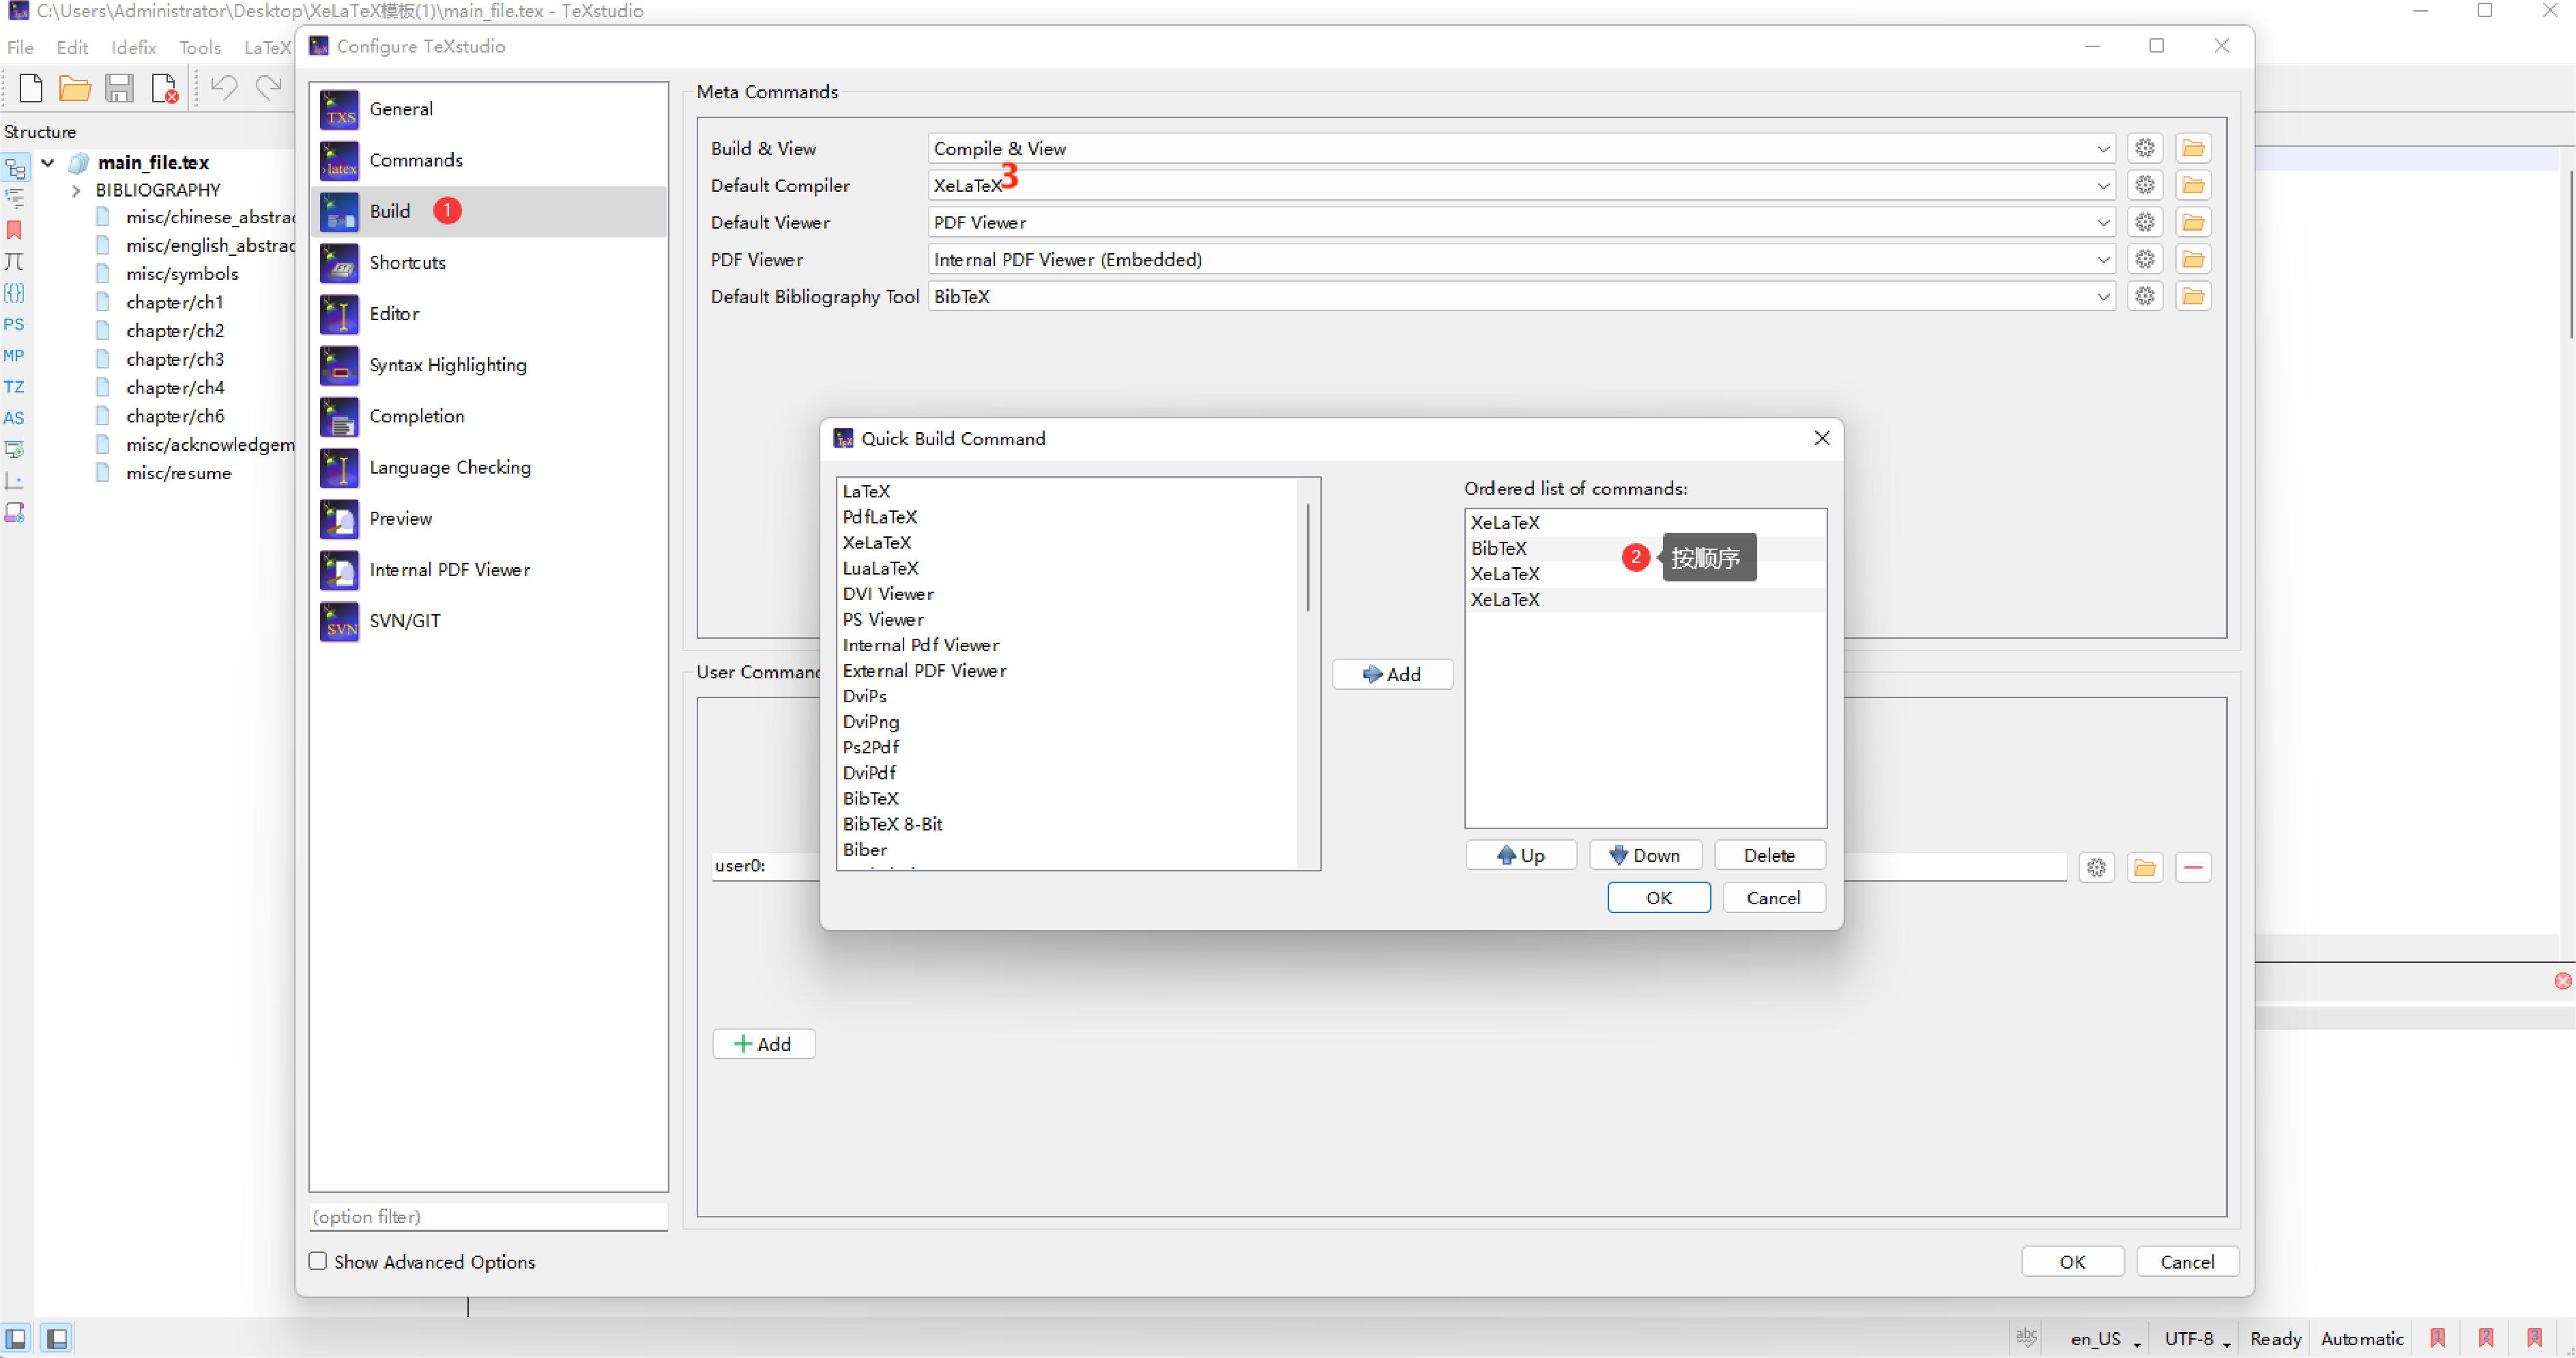
\includegraphics[width = \textwidth]{a1.pdf}
	\bicaption{编译方式设置}{Compilation mode setting}
	\label{fig_0}
\end{figure}

点击工具——用户进行编译,如图\ref{fig_1}所示。

\begin{figure}[htbp]
	\centering
	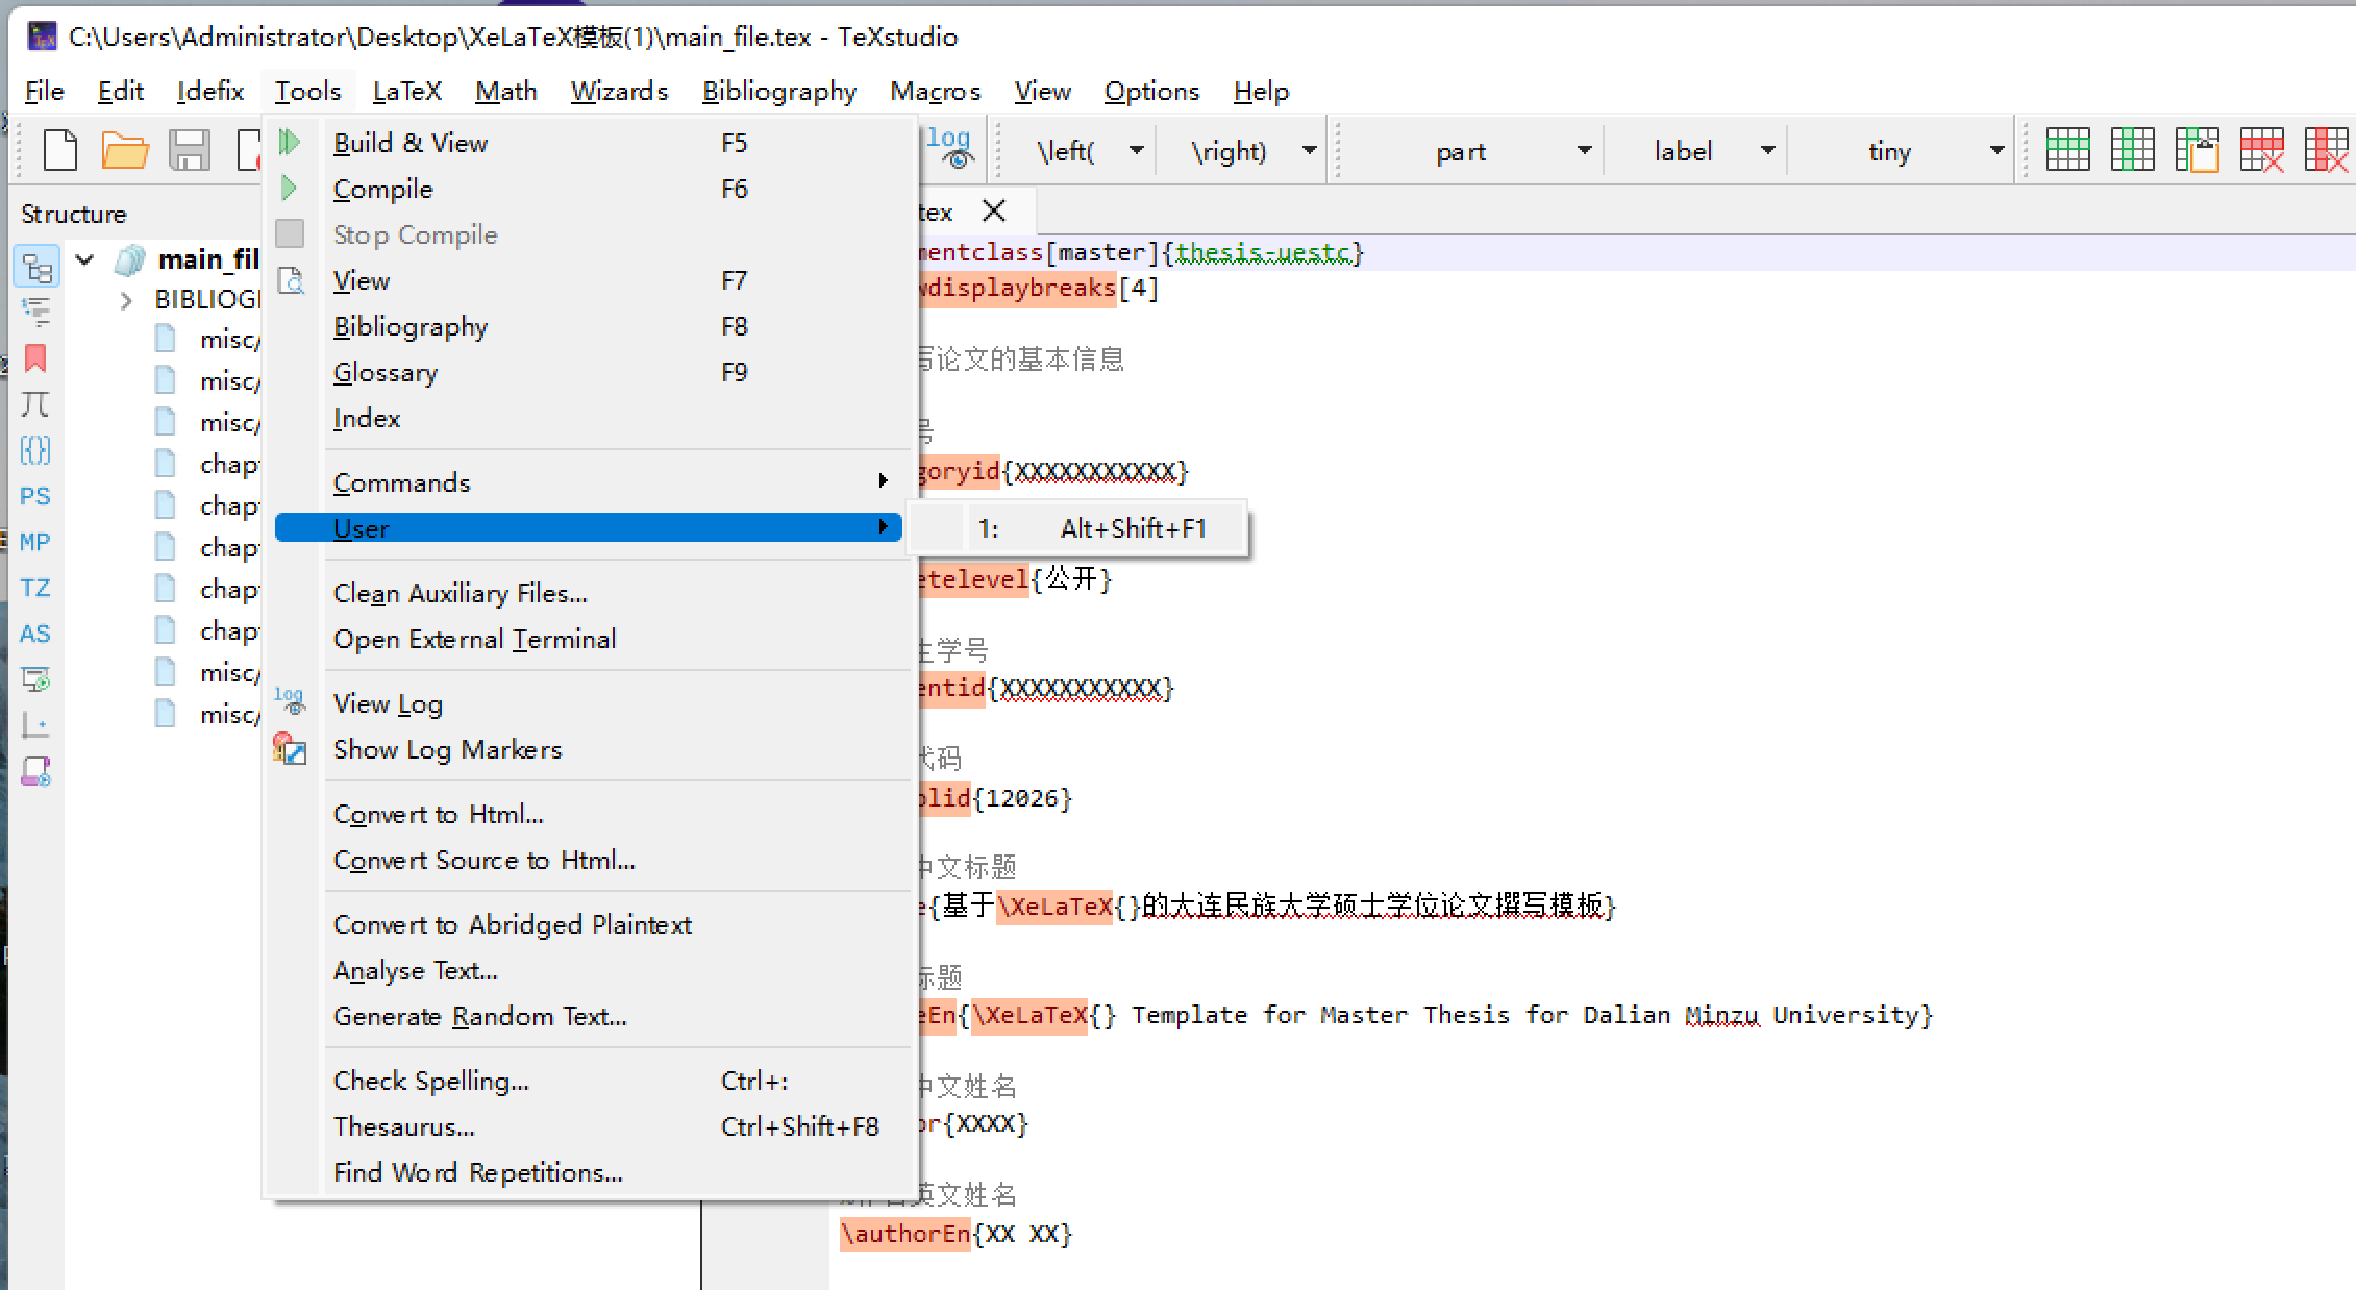
\includegraphics[width = \textwidth]{a2.pdf}
	\bicaption{编译方式设置}{Compilation mode setting}
	\label{fig_1}
\end{figure}

\section{latex安装教程}
本节将介绍本模板的一些设置内容以及基本使用方法,下载地址:

1) TexLive官网:\href{https://mirrors.tuna.tsinghua.edu.cn/CTAN/systems/texlive/Images/}{https://mirrors.tuna.tsinghua.edu.cn/CTAN/systems/texlive/Images/};

2) TeXstudio官网:\href{https://texstudio.sourceforge.net/}{https://texstudio.sourceforge.net/};

3)
 详细安装方式请见:\href{https://blog.csdn.net/weixin_43872190/article/details/113736283?spm=1001.2014.3001.5502}{详细地址}。


\section{字体安装}
在本字体文件夹里,先将这四种字体进行全局安装,右键——为所有用户安装
如图\ref{fig_2}所示。

{\tiny \begin{figure}[htbp]
	\centering
	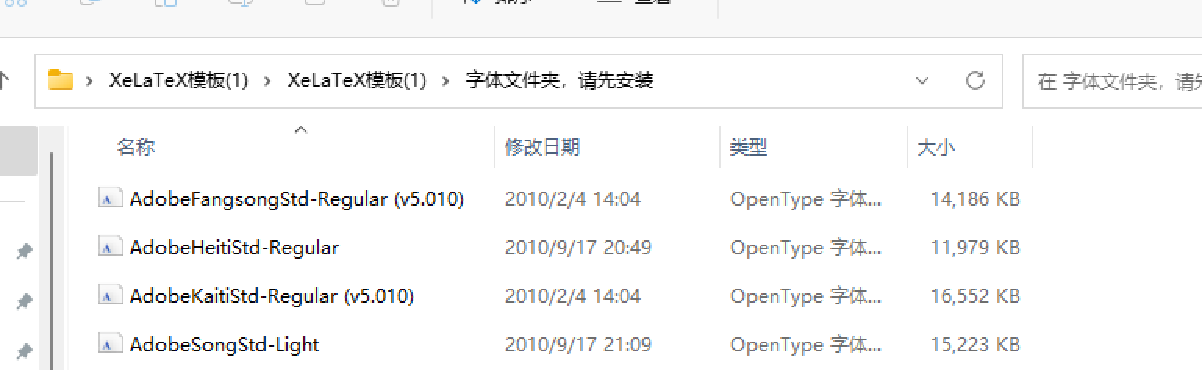
\includegraphics[width = \textwidth]{a3.pdf}
	\bicaption{字体安装}{Font installation}
	\label{fig_2}
\end{figure}}

注:

1)运行latex后右边自动显示pdf;

2)按住ctrl双击也可显示pdf;

3)按住ctrl双击右边pdf可以跳转到对应的latex代码。



\end{document}        %第一章 绪论
\documentclass{standalone}
% preamble: usepackage, etc.
\begin{document}

\chapter{latex设置说明}

(注意段落标题之间不能有空白必须有正文)(注意段落标题之间不能有空白必须有正文)(注意段落标题之间不能有空白必须有正文)(注意段落标题之间不能有空白必须有正文)(注意段落标题之间不能有空白必须有正文)

\label{chap2}

\section{语言模式}

本模板只有一套中文基础语言环境。改变语言环境会改变图表标题的引导词(图,表),文章结构词(比如目录,参考文献等),以及定理环境中的引导词(比如定理,引理等)。段落等文字直接粘贴即可,格式均自动调整。

\section{标题设置}
以下为各级标题格式:

1) {chapter}为一级标题提示符;

2)  {section}为二级标题提示符;

3)  {subsection}为三级标题提示符。

\section{图片设置}
{figure}为插入图片提示符,本latex所使用的图片应为矢量图格式,即.pdf格式。
由于插入的图片为.png或.jpg时可能会出现图片不清晰,缩放会失真,将图片转换为矢量图可编辑性更好,更适合印刷。

\subsection{图片格式转换}

尽量使用微软visio和Adobe AI等软件制作矢量图,新版模版论文支持矢量图,打印和放缩都会清晰不失真。如果不会只用JPG,可以将.jpg或者.png文件转换为.pdf格式的详细方法:

1)将.jpg或者.png文件上传到\href{https://img.logosc.cn/?utm_source=zhihutg05.com/}{https://texstudio.sourceforge.net/},点击AI改图——文件格式转换,选择转换方式为pdf,点击下载完成;

2)如果失效,请点击:\href{https://www.zhihu.com/question/292896684}{https://texstudio.sourceforge.net/}。


\subsection{图片引用}
label为图片引用标签,如图\ref{fig_20}所示。
\begin{figure}[htbp]
	\centering
	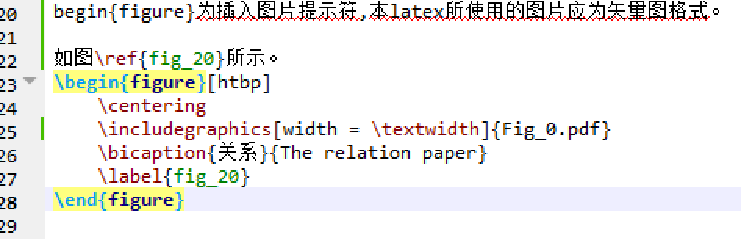
\includegraphics[width = \textwidth]{a11.pdf}
	\bicaption{图片引用方式}{Image reference mode}
	\label{fig_20}
\end{figure}



\section{公式引用}\label{sec_face_landmark}
 
 文中所有外文计量单位(如千克kg)、固定标准函数(如三角函数)、事物名称、数字、数学运算符等用正体,外文变量或物理量、非固定标准函数都用斜体,向量、集合、矩阵、张量用粗斜体(上下标不用加粗)。

语言的使用过程是人们在受语言内部或者外部因素的驱动下有意无意不断进行语言选择的过程$E_1, E_2, \dots,E_n, \dots, E_{N_E}$和一个门控神经网络$G$所组成的。

\begin{equation}
	a = - \sum_{i=1}^{n}{y_i\:\log(\hat{y_i})} +     \label{eq:0}
	\lambda {\left\lVert\omega\right\rVert}_2^2
\end{equation}


\begin{equation}\label{eq_fs_parameter}
	b_{j} = \left\{\begin{array}{lcl}
		f_{j} & \text{if} & k=1\\ 
		f_{i} & \text{if} & k=N_{fs}
	\end{array}\right.
\end{equation}


商讨性和顺应性三个相互关联的本质属性。因此,式(\ref{eq_fs_parameter})为所引用公式,两者名称应一致,如图\ref{fig_11}。

\begin{figure}[htbp]
	\centering
	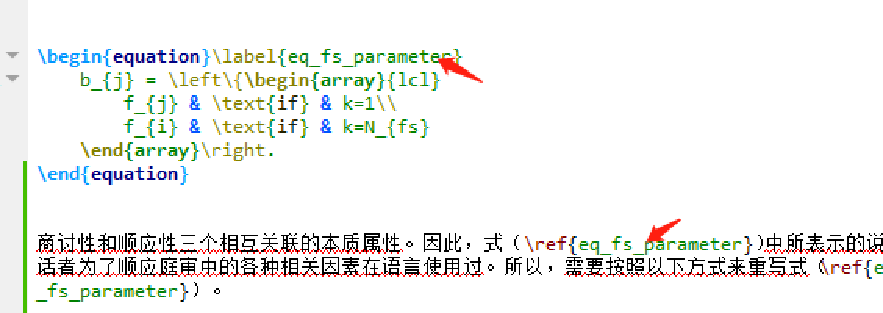
\includegraphics[width = \textwidth]{a12.pdf}
	\bicaption{公式引用}{The relation paper}
	\label{fig_11}
\end{figure}

更多相关公式的例子请参考:\href{https://zhuanlan.zhihu.com/p/110756681}{https://zhuanlan.zhihu.com/p/110756681}


\end{document}
        %第二章
\documentclass{standalone}
% preamble: usepackage, etc.
\begin{document}
\chapter{表格引用}
\section{表格引用}
以下为表格引用格式:

1) table为插入表格提示符;

2) bicaption为表格标题提示符;

3) tabular及后面大括号为表格的列;

4) hline为表格行添加的横线(一般为三线表)。


\begin{table}[htbp]
	\renewcommand{\arraystretch}{0.75}
	\bicaption{数据集}{Datasets Analysis}
	\label{tab_dataset}
	\setlength{\tabcolsep}{1pt}
	\centering 
	\begin{tabular}{lccccccc}
		\hline
		数据集 & \#p. & \#i. & \#c. & \%M. & \#A.\\
		\hline
		A & 48 & 1 & 2 & 67 & \textsl{AU}\\
		Au & 60 & 4 & 2 & 5.5 & \textsl{AU}\\
		B & 625 & 4 & 3 & 4.1 & \textsl{BL}\\  
		W & 49 & 5 & 2 & 94.6 & \textsl{T}\\
		\hline
	\end{tabular}
\end{table}

\section{algorithm算法使用}
以下为algorithm算法的使用方式:

1) caption为算法的标题;

2) label为算法的标签,方便在文章中引用;

3) REQUIRE为算法的输入;

4) ENSURE为算法的输出。


\begin{algorithm}[htbp]
	\caption{语言的艺术中生成模糊规则}
	\begin{algorithmic}[1]
		\REQUIRE \;\\
		$X_{tr} ={a}$,样本集;\\
		$Y_{tr} ={b}$,标签集;\\
		\ENSURE \;\\
		$\bm{B} = (b_{k})$,矩阵;\\
		$\bm{P} = (p_{l})$,概率。 
		\FOR{$j = 1$ to $N_{f}$}
		\FOR{$k = 1$ to $N_{fs}$}
		\STATE 通过式(\ref{eq_fs_parameter})获取$b_{j}$;
		\ENDFOR
		\ENDFOR
	\end{algorithmic}
	\label{alg_iwm_train}
\end{algorithm}



\section{定义引用}

本节为定义定理类的引用,definition为定理提示符,label为定义的标签,方便在文章中引用,enumerate为条件提示符,item表示第几点,如图\ref{fig_13}所示。

引用定义\ref{def_neighbour}的条件得出结论。

\begin{definition}\label{def_neighbour}
	对于$\forall s_{i} \in S$, 满足以下条件:
	\vspace{-3pt}
	\begin{enumerate}
		\item $\bm{a} = (p_{i})$
		\item $\bm{P} = (p_{3})$
	\end{enumerate} 
\end{definition}

\begin{figure}[htbp]
	\centering
	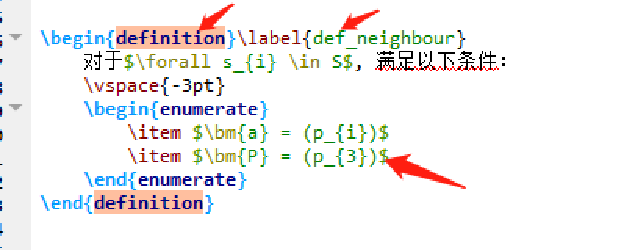
\includegraphics[width = \textwidth]{a15.pdf}
	\bicaption{定理引用教程}{Theorem reference tutorial}
	\label{fig_13}
\end{figure}

\end{document}        %第三章
\documentclass{standalone}
% preamble: usepackage, etc.
\begin{document}
\chapter{BIB参考文献数据及软件使用}

(注意段落标题之间不能有空白必须有正文)(注意段落标题之间不能有空白必须有正文)(注意段落标题之间不能有空白必须有正文)(注意段落标题之间不能有空白必须有正文)(注意段落标题之间不能有空白必须有正文)

\label{chap4}

\section{JabRef安装}
以下为JabRef安装的安装方式:

1)安装地址:\href{https://www.jabref.org/}{官网地址,点击跳转};

2)点击download,如图\ref{fig_3}所示;
\begin{figure}[htbp]
	\centering
	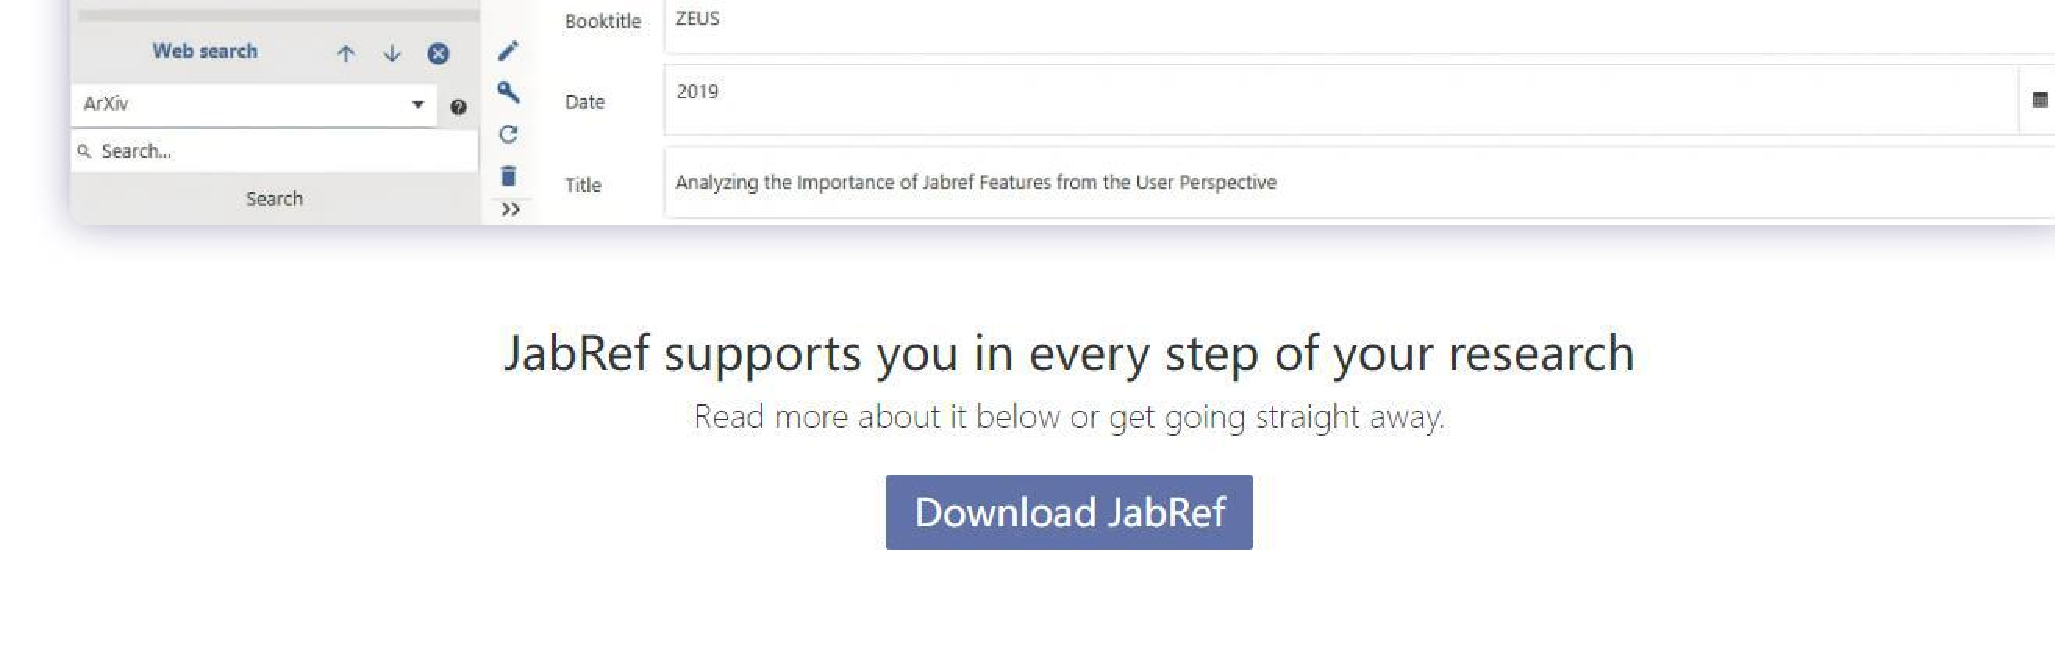
\includegraphics[width = \textwidth]{a4.pdf}
	\bicaption{安装方式}{Installation mode}
	\label{fig_3}
\end{figure}

3)双击JabRe图标按提示进行安装,如图\ref{fig_4},安装完成后无需进行Java环境变量的配置;
\begin{figure}[htbp]
	\centering
	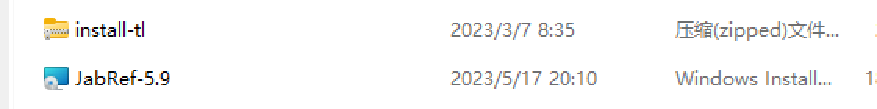
\includegraphics[width = \textwidth]{a5.pdf}
	\bicaption{直接安装}{Direct installation}
	\label{fig_4}
\end{figure}

4)设置中文模式:Options-> Preference-> General,设置语言为“中文简体”。


\section{使用方法}
以下为JabRef的使用方法:

1)文件——新建库——ctrl+s保存,选择一个文件夹放进去,进行命名,如图\ref{fig_5};
\begin{figure}[htbp]
	\centering
	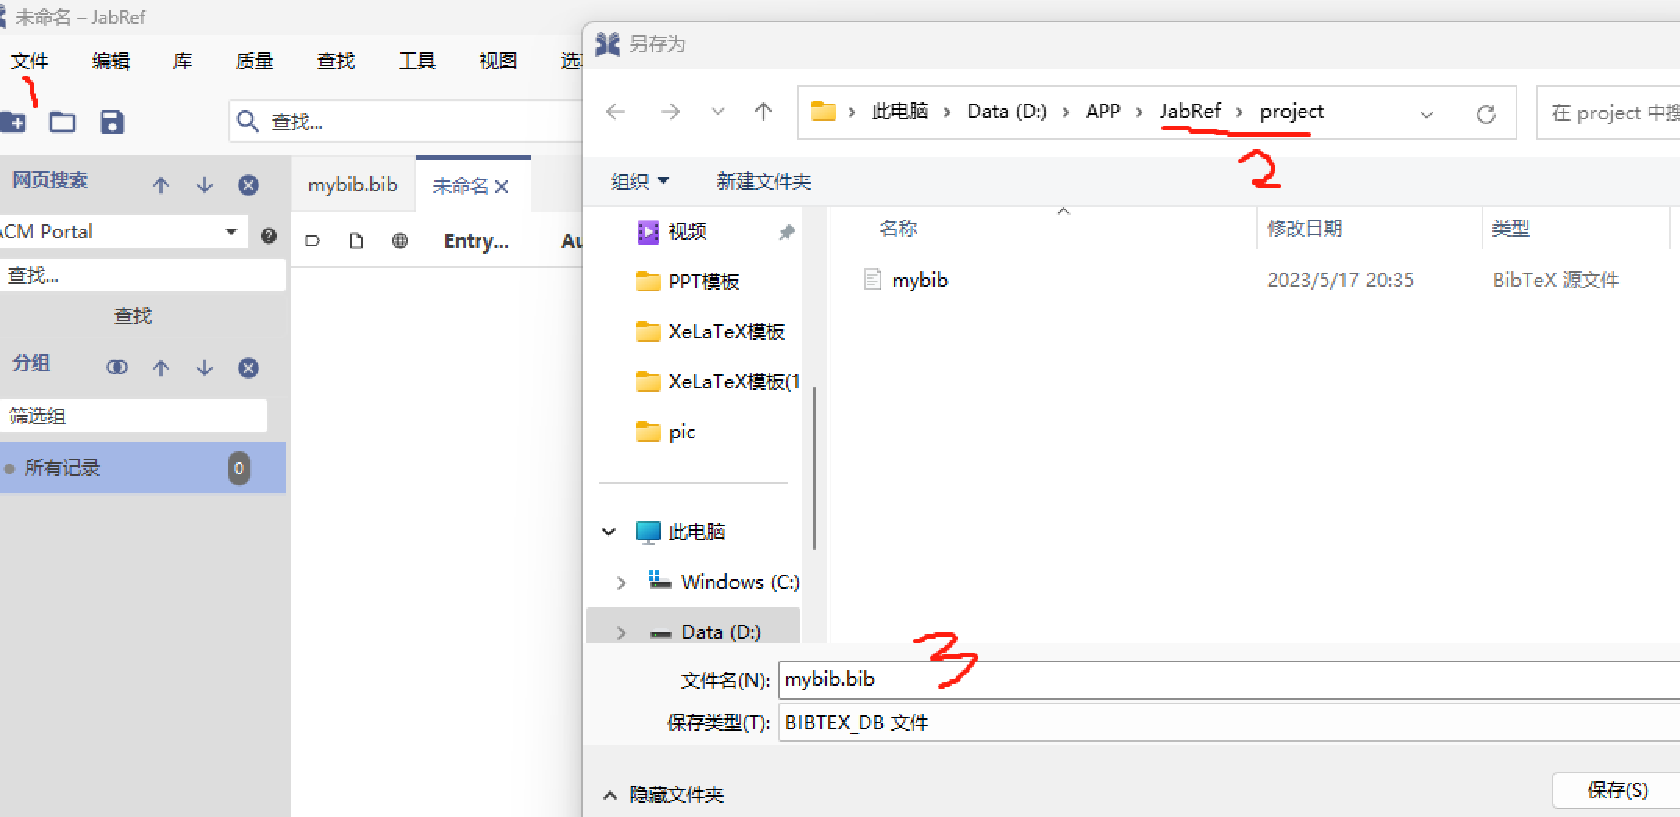
\includegraphics[width = \textwidth]{a6.pdf}
	\bicaption{保存文件}{Save file}
	\label{fig_5}
\end{figure}

2)添加参考文献:新建一个article,点击图标栏的这个加号,如图\ref{fig_7},
\begin{figure}[htbp]
	\centering
	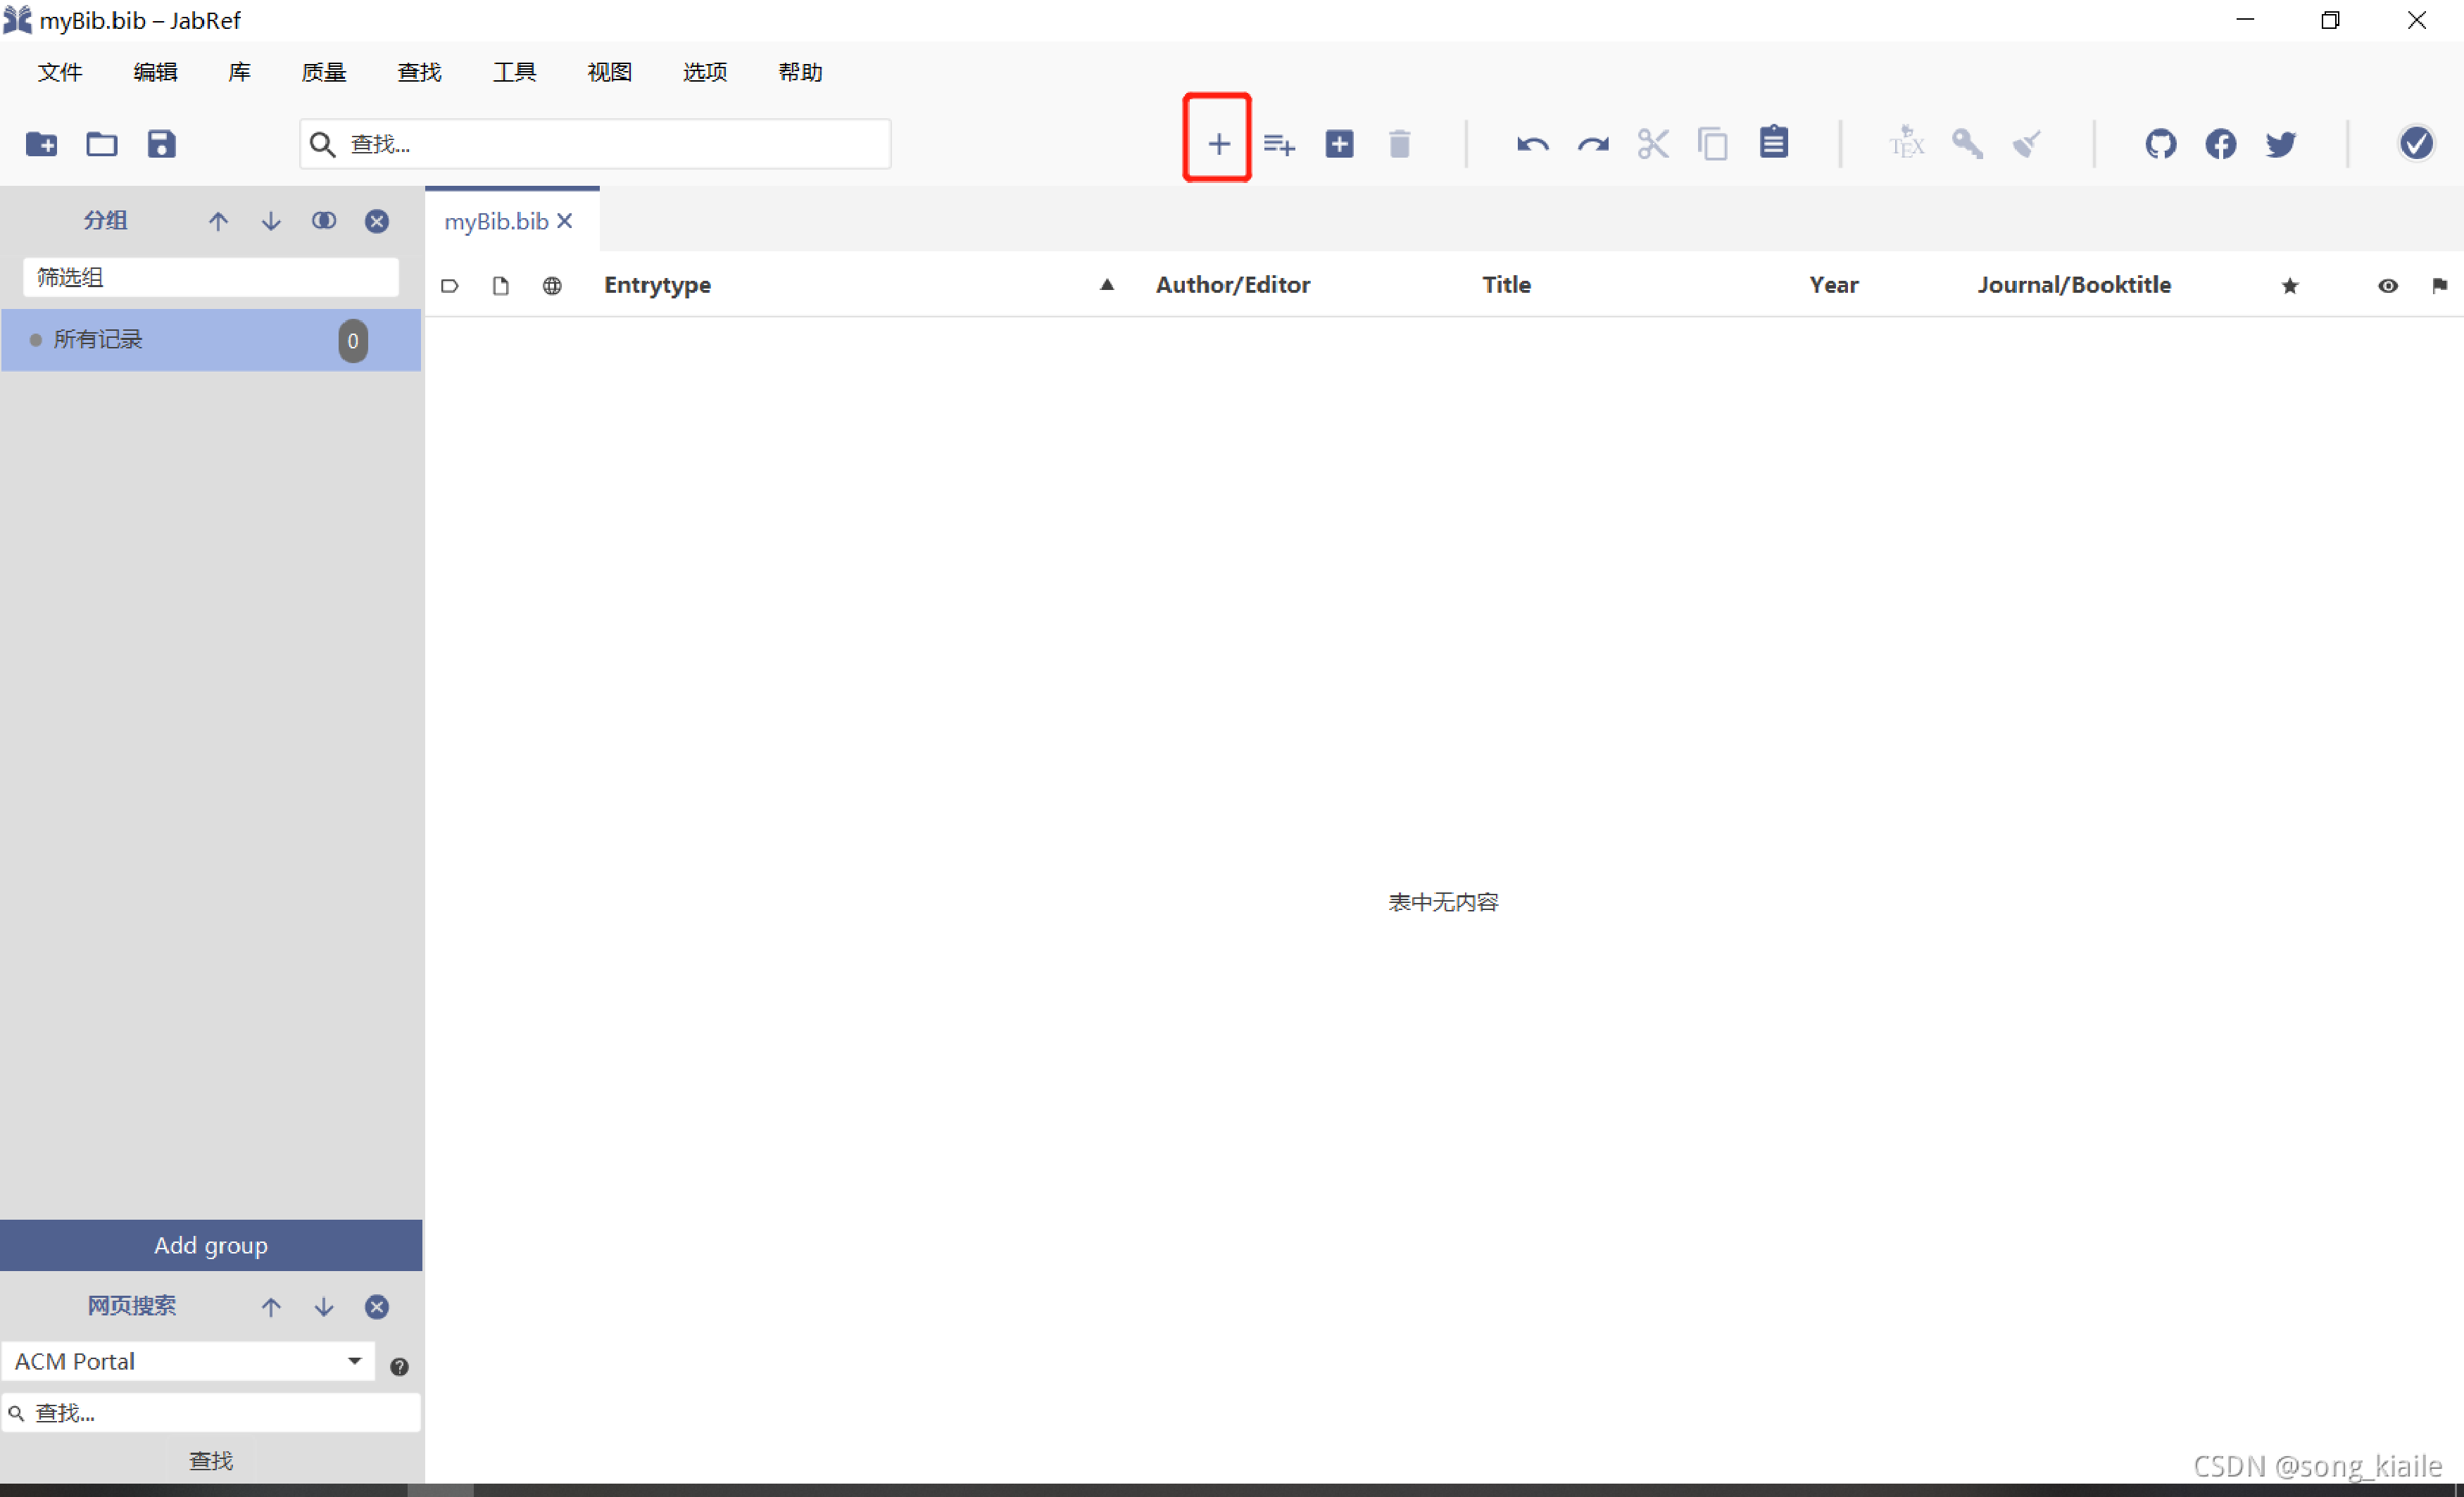
\includegraphics[width = \textwidth]{a8.pdf}
	\bicaption{新建文件}{New file}
	\label{fig_7}
\end{figure}
设置成功后如图\ref{fig_6}所示;
\begin{figure}[htbp]
	\centering
	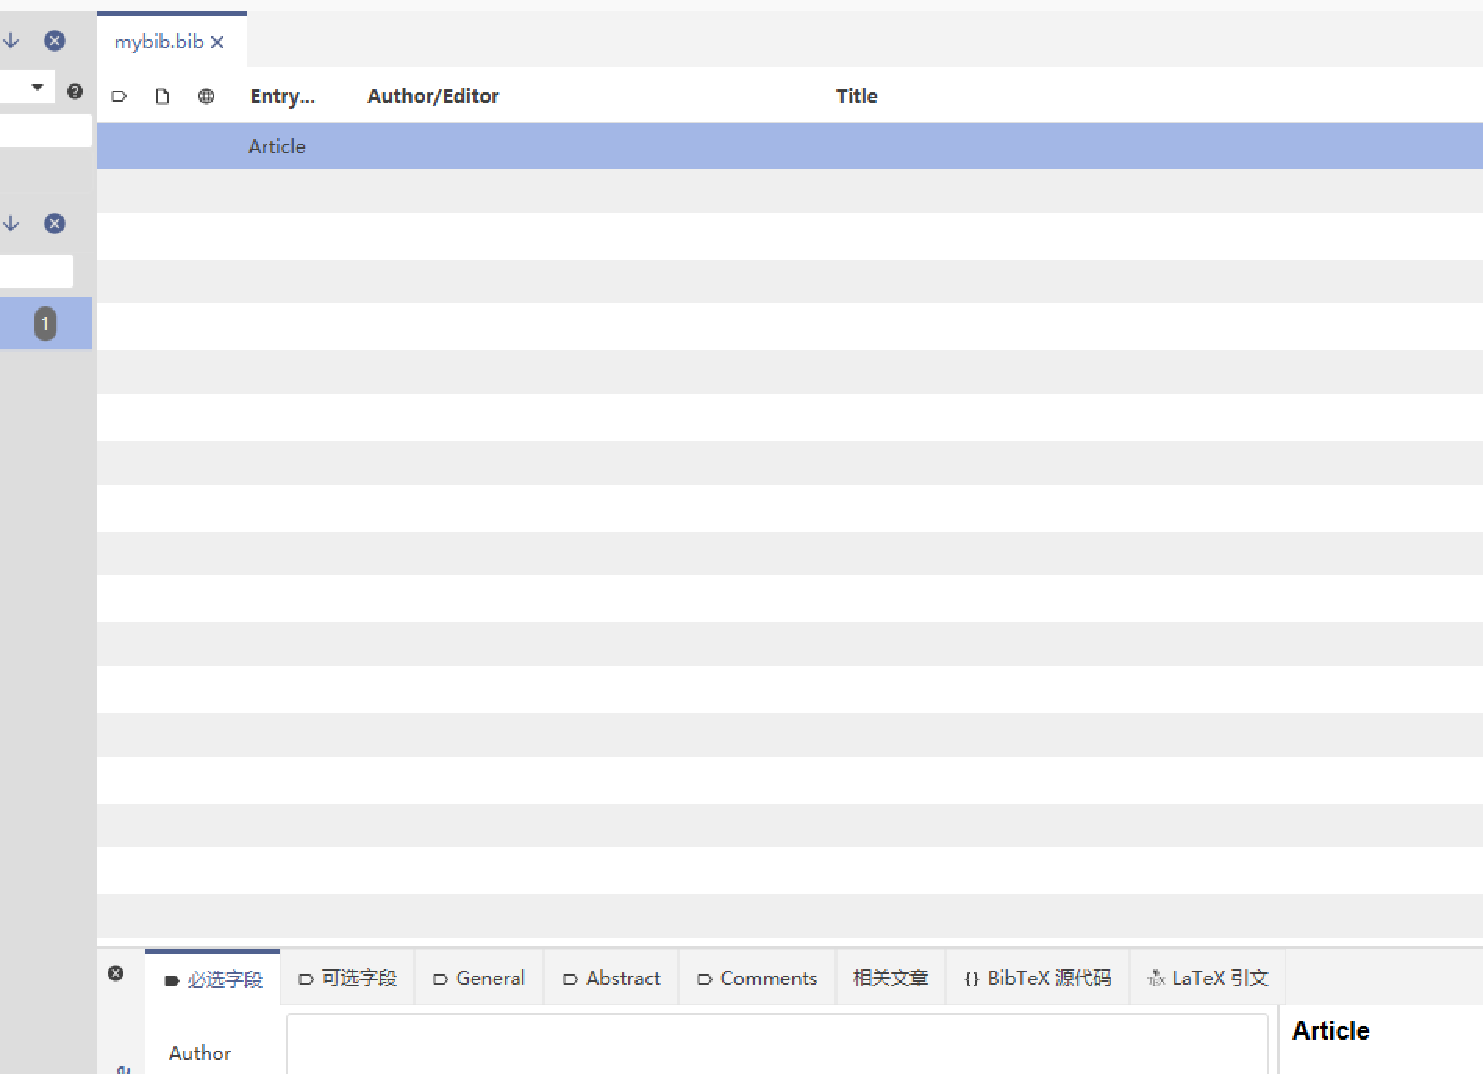
\includegraphics[width = \textwidth]{a7.pdf}
	\bicaption{新建成功界面}{Creating a successful screen}
	\label{fig_6}
\end{figure}

3)谷歌学术随便搜一个文献,复制BibTex,粘贴到下面这个区域,如图\ref{fig_8},然后保存就可以了;
\begin{figure}[htbp]
	\centering
	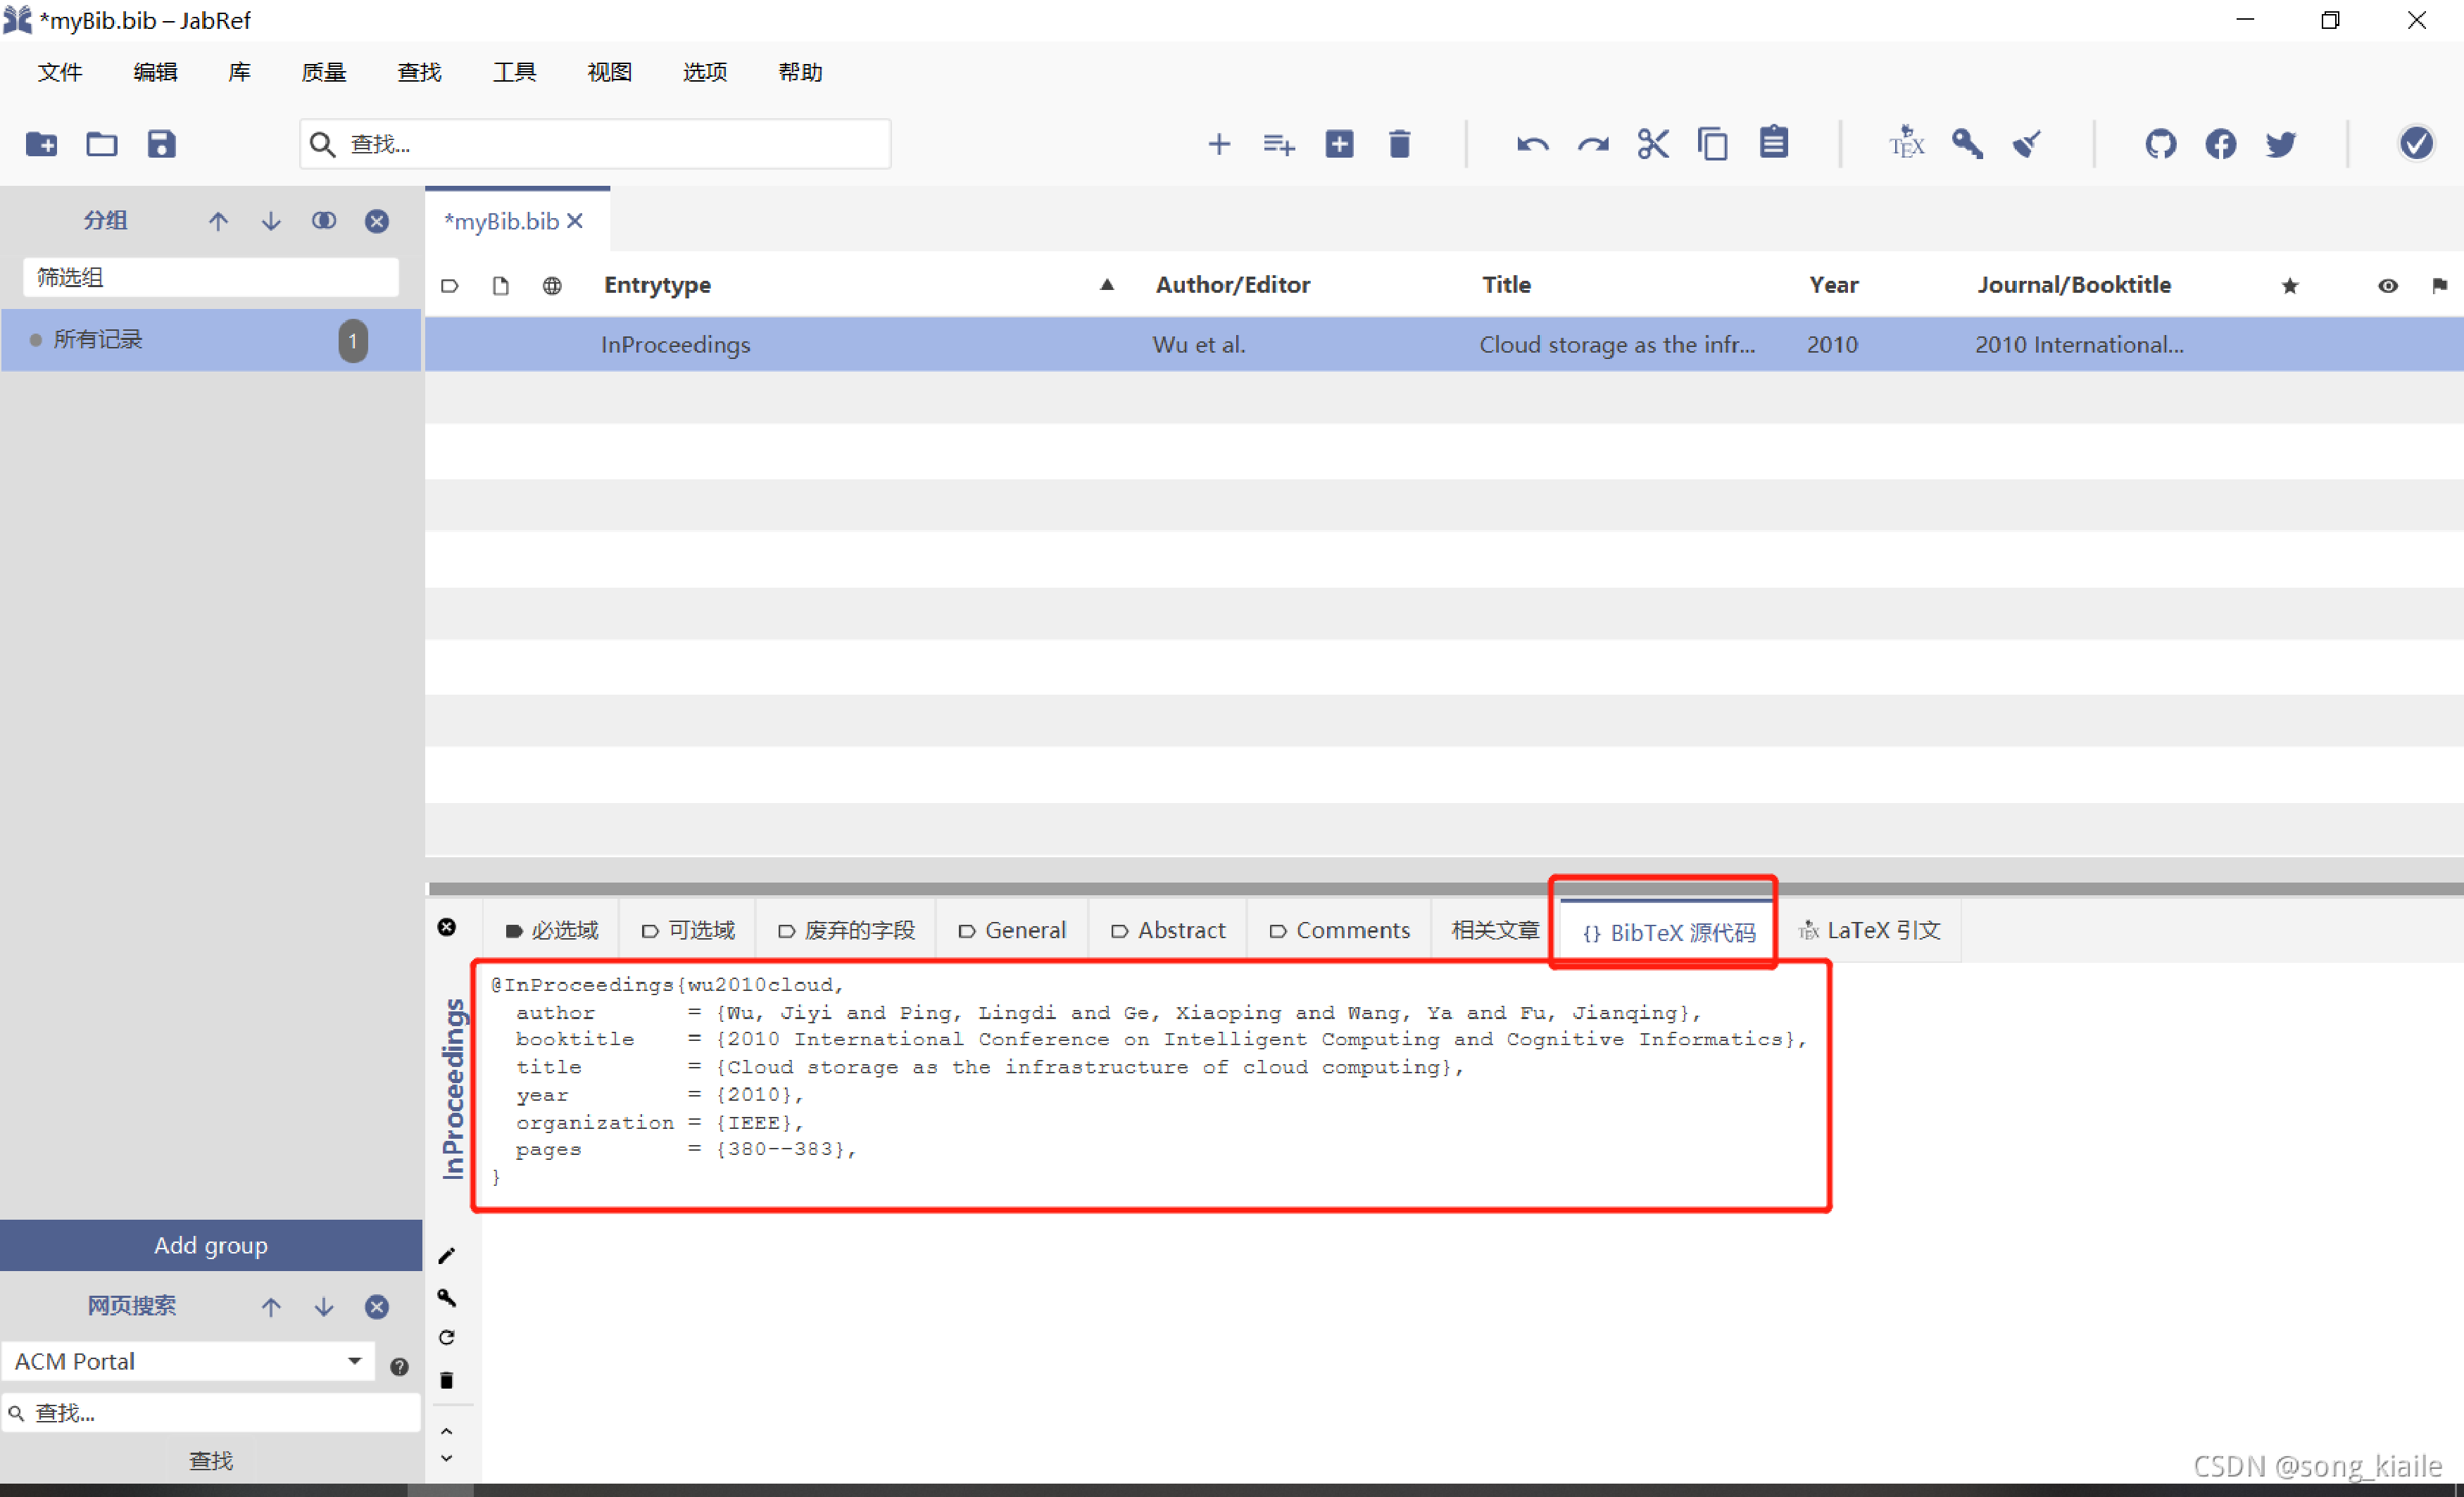
\includegraphics[width = \textwidth]{a9.pdf}
	\bicaption{参考文献界面}{Reference interface}
	\label{fig_8}
\end{figure}

4)可以看到“必选域”这里已经有了作者,标题,年份等信息,如图\ref{fig_9};
\begin{figure}[htbp]
	\centering
	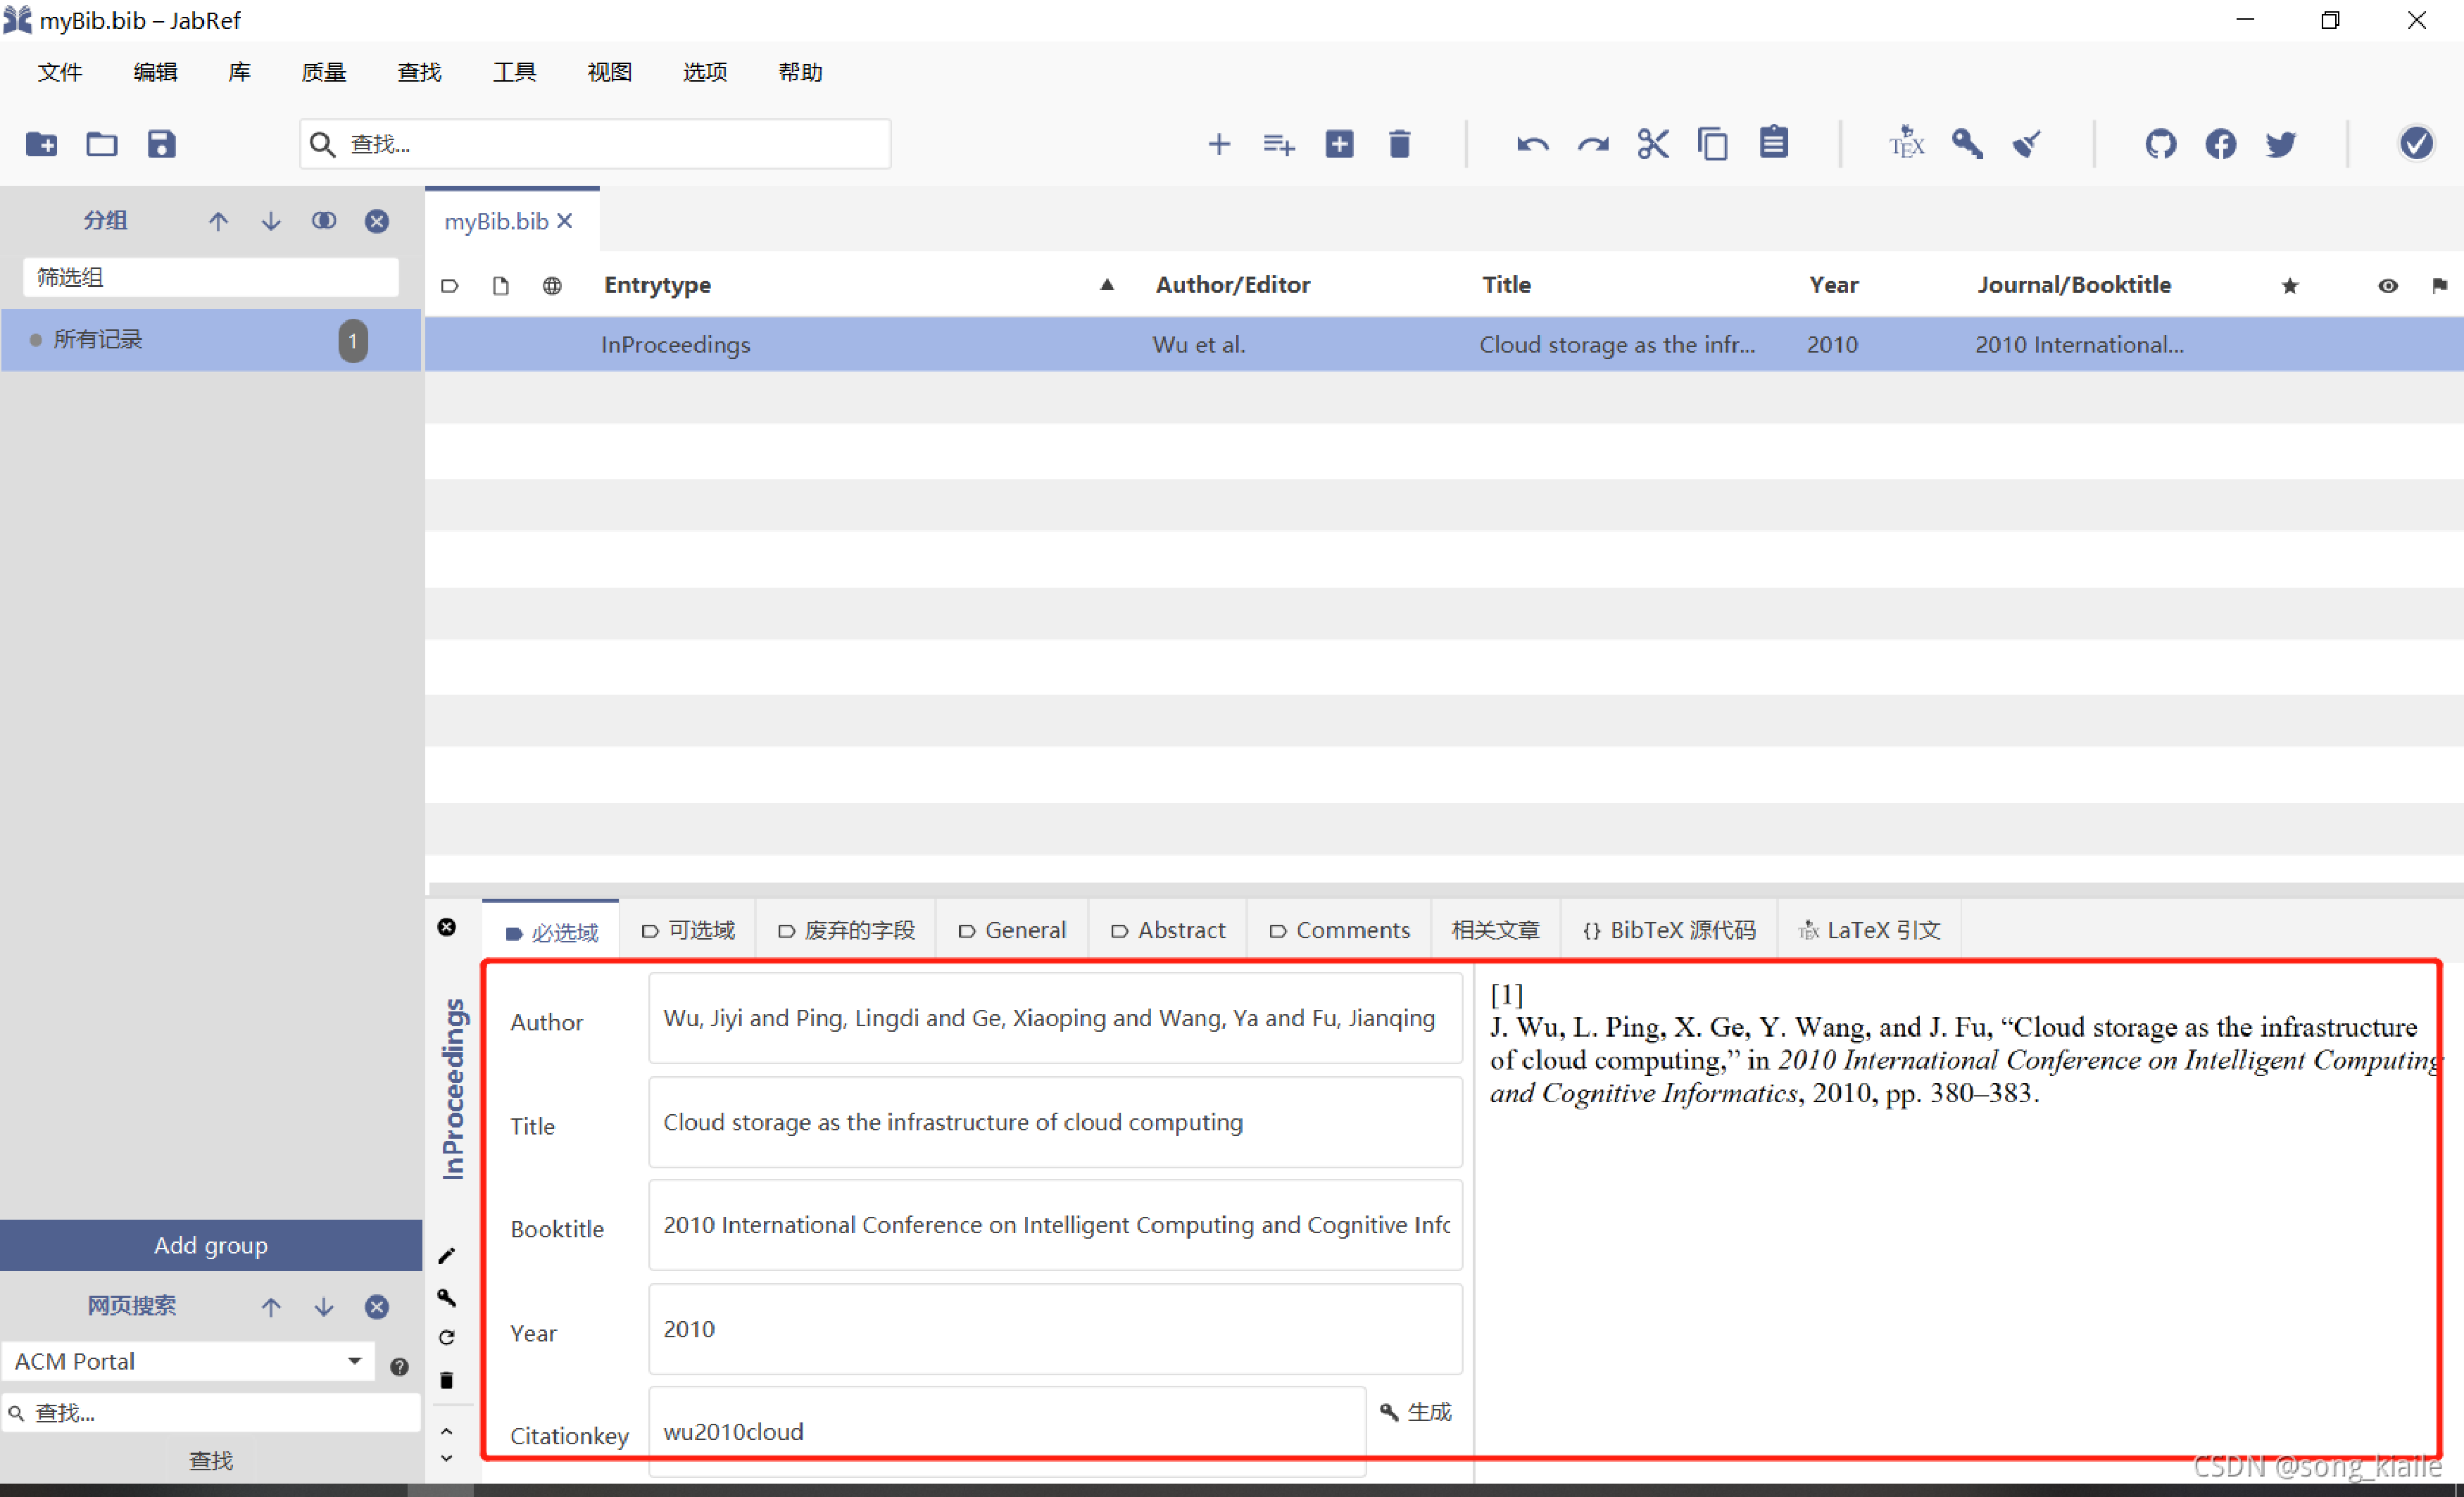
\includegraphics[width = \textwidth]{a10.pdf}
	\bicaption{参考文献}{Reference}
	\label{fig_9}
\end{figure}

5)最后将BibTex源代码粘贴到reference参考文献里面。


\section{文献引用}

1)添加文献:可以通过手动输入文献信息、导入文献文件或者通过DOI号码添加文献;

2)组织文献:可以通过添加关键词、标签、笔记等方式对文献进行分类和组织;

3)搜索文献:可以使用JabRef内置的搜索功能快速找到需要的文献,如图\ref{fig_10}所示;
	\begin{figure}[htbp]
		\centering
		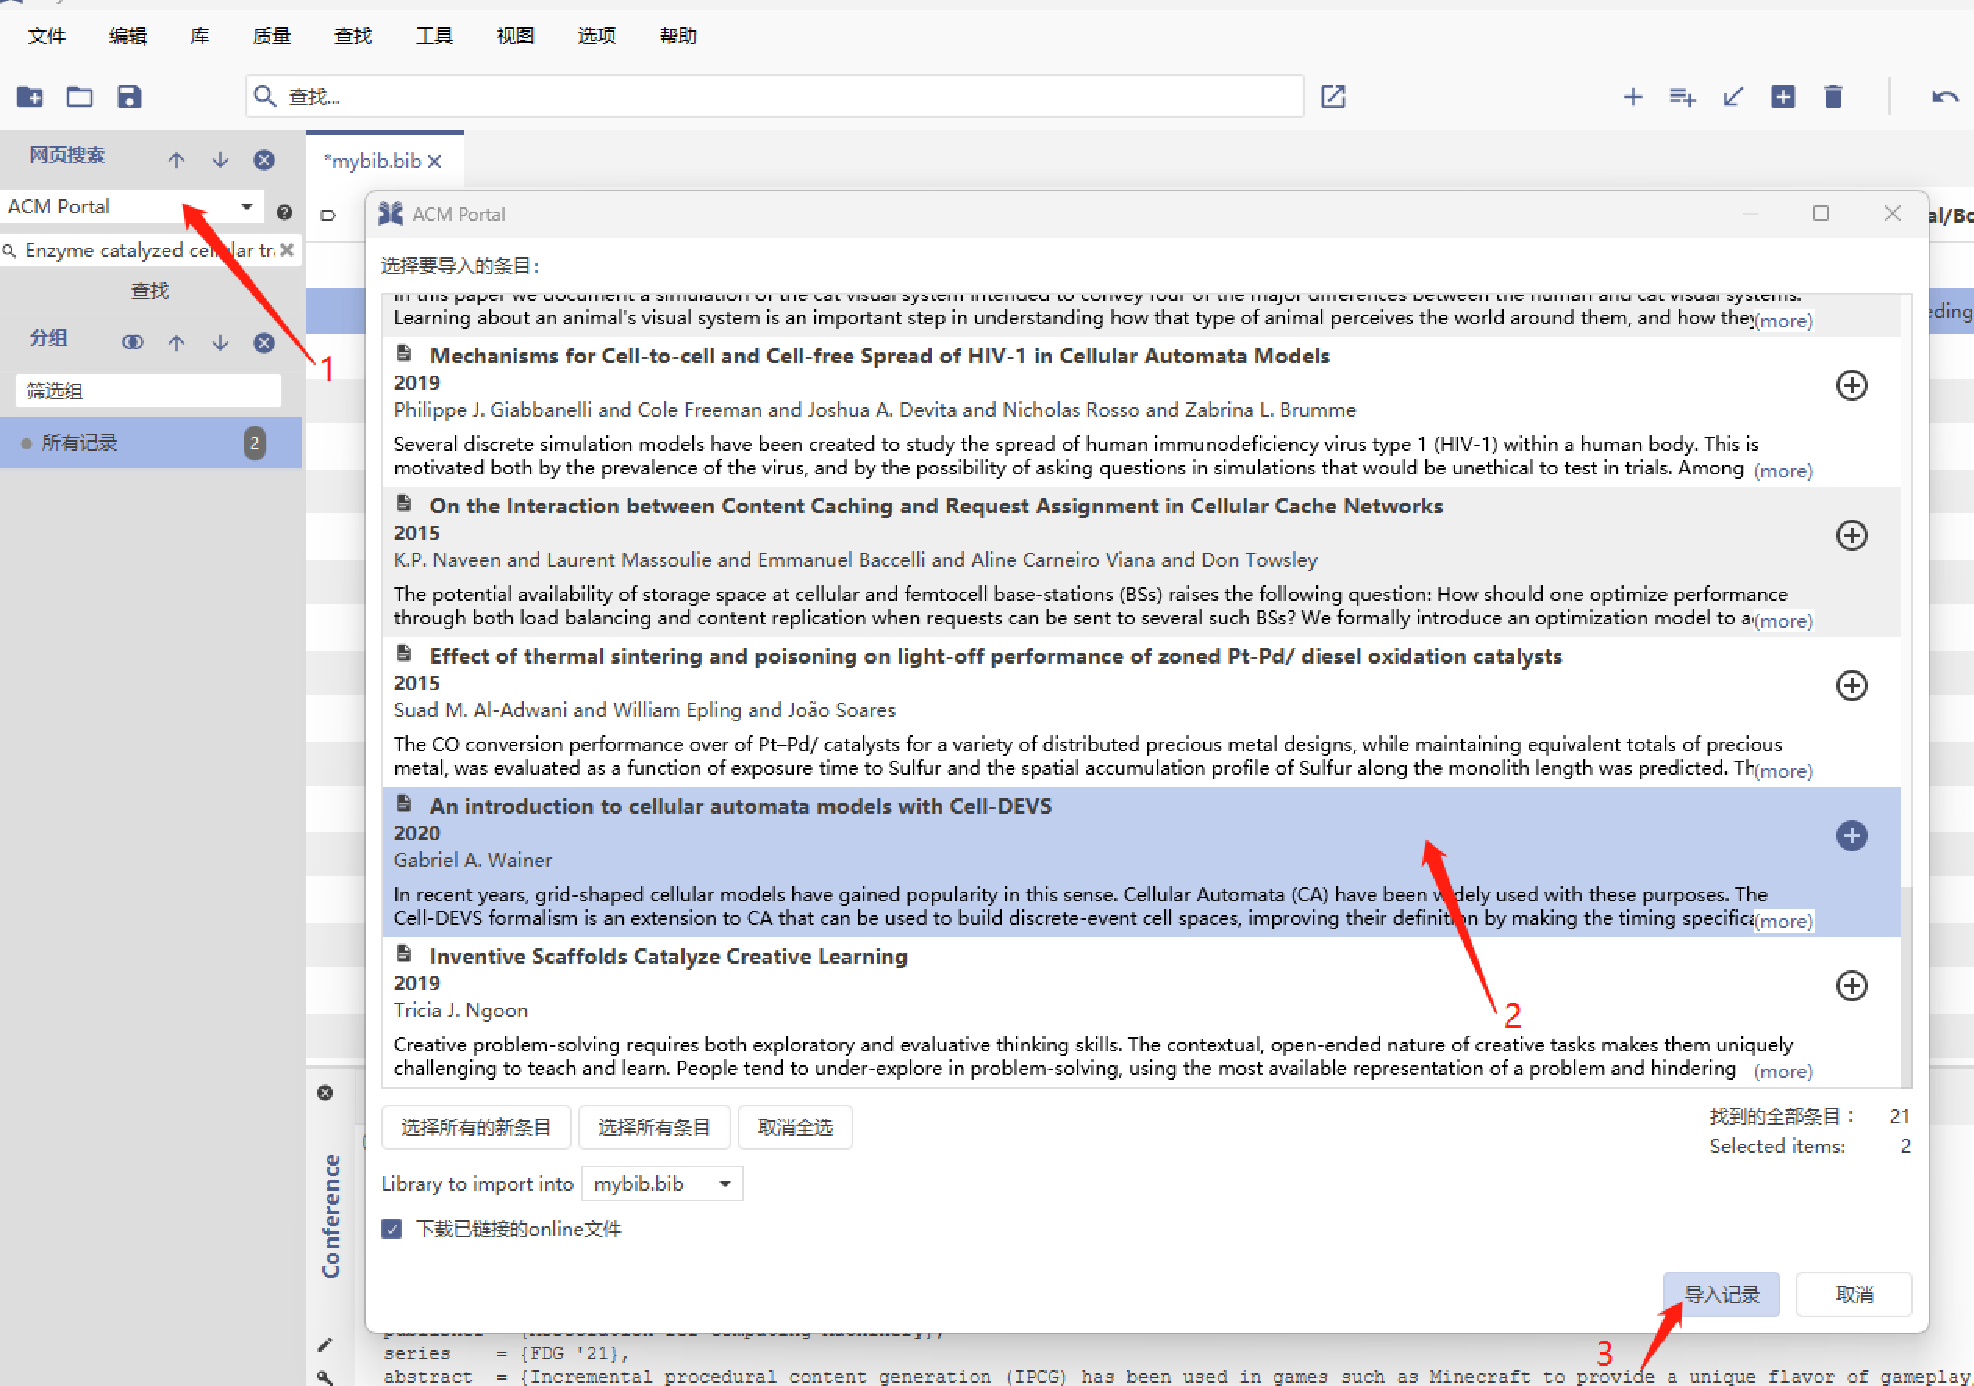
\includegraphics[width = \textwidth]{a13.pdf}
		\bicaption{搜索文献}{Search literature}
		\label{fig_10}
	\end{figure}
	
4)导出文献:可以将选定的文献导出为各种格式,如BibTeX、EndNote、RIS等;

5)连接文献库:可以将JabRef与外部文献数据库(如PubMed、Google Scholar等)连接,以便自动获取文献信息;

6)插入引用:可以在写作时轻松插入引用,并自动生成参考文献列表。

以上是JabRef基本使用教程的简要介绍,更多详细操作请参考JabRef的官方文档或其他相关资料。

\section{参考文献}

(注意段落标题之间不能有空白必须有正文)文献这里最好用google学术,把论文的卷、期和页面查准,如果不全,生成的也会缺失。

\subsection{参考文献引用方法}

上面的箭头为本文件reference粘贴过来的Bib参考文献,下面的箭头为引用方式,两者名称一致,如图\ref{fig_12}。每一次添加文献都需要按图\ref{fig_1}所示的编译方法编译,否则编译不成功,无法正确引用参考文献。
\begin{figure}[htbp]
	\centering
	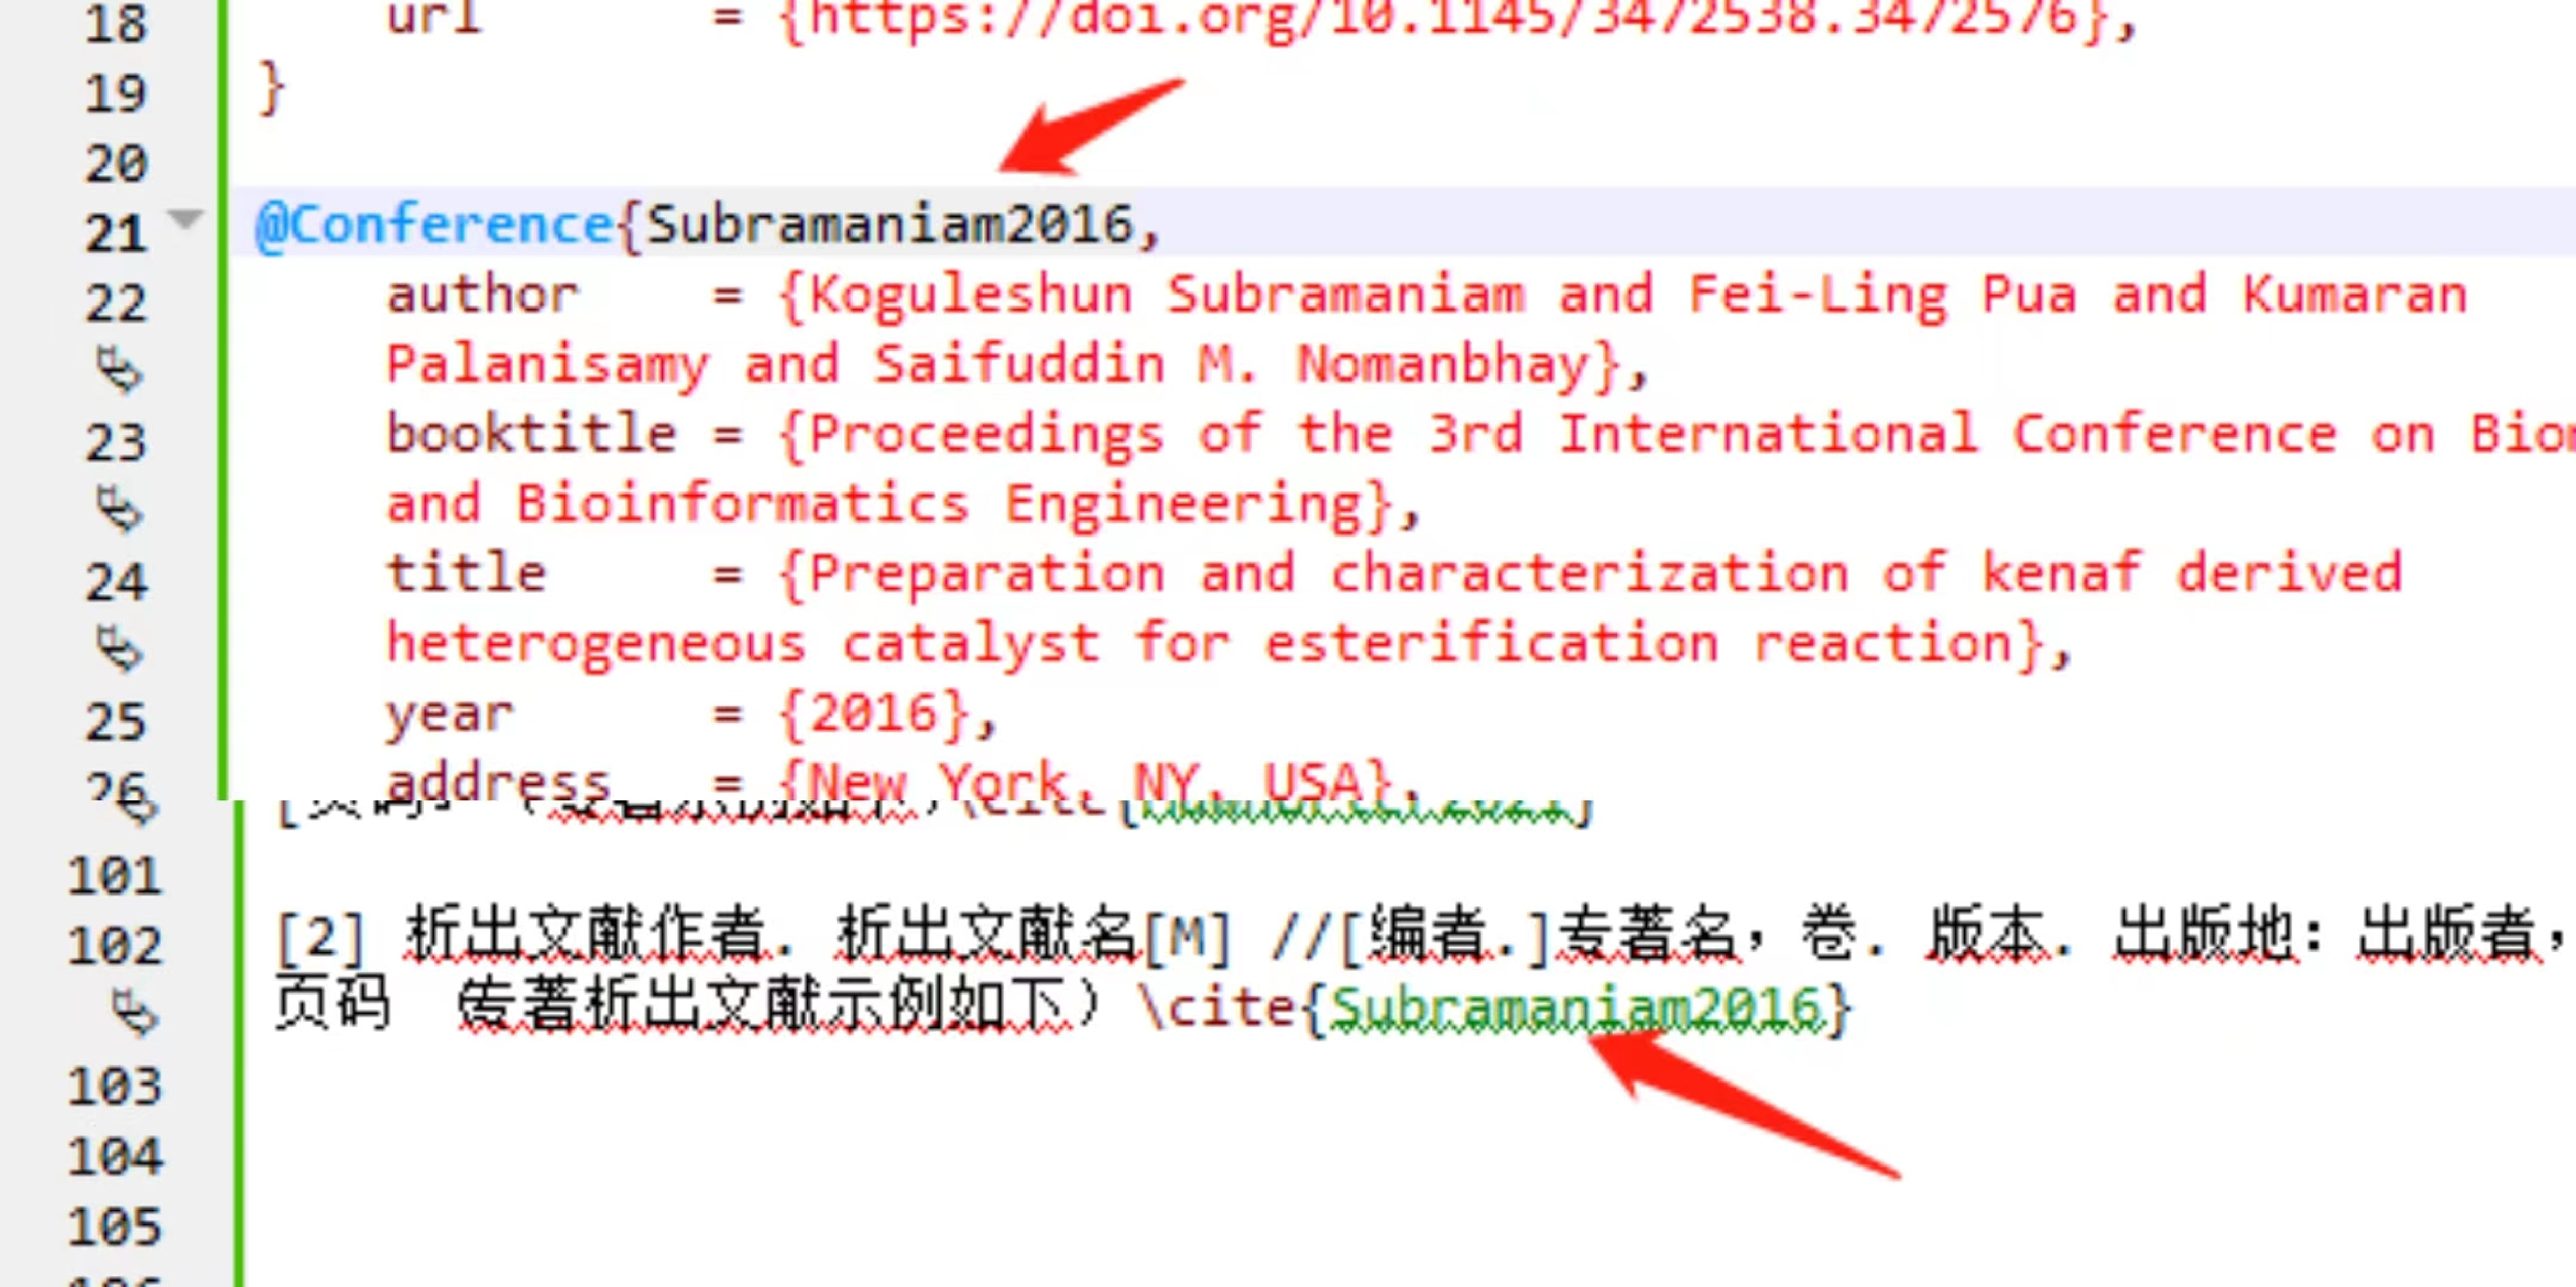
\includegraphics[width = \textwidth]{a14.pdf}
	\bicaption{引用方法}{Reference method}
	\label{fig_12}
\end{figure}

注:author如果有多个,中间用and连接,否则会出错。



\subsection{参考文献引用示例}
[1]	作者. 书名[M].  版本(第1版不注). 出版地:出版者,出版年: [页码](专著示例如下)\cite{Mawhorter2021}

[2]	析出文献作者. 析出文献名[M] //[编者.]专著名,卷. 版本. 出版地:出版者,出版年: 页码 (专著析出文献示例如下) \cite{Subramaniam2016}

[3]	原作者. 原文书名[M]. 出版地:出版者,出版年:页码(in Chinese) (译著示例如下) \cite{ref_1}

[4]	用户手册名[M]. 出版地:出版者,出版年 (用户手册示例如下) \cite{ref_2}

[5]	作者. 题名[J]. 期刊名,年,卷(期):页码//作者. 题名[N]. 报纸名,年-月-日(版次)(连续出版物示例如下) \cite{ref_3}

[6]	作者. 题名[J/OL].期刊名,年,卷(期):页码[引用日期]. 获取和访问路径其中引用日期用投稿日期替换即可。(连续出版物中的析出文件,以期刊为例示例如下) \cite{ref_4}

[7]	作者. 题名[C](后面无句号) //会议论文集名称。出版地:出版者,出版年:页码(若是英文文献,英文会议论文集的题目请以“Proceedings(此处有s) of …开始,每个单词全拼,每个实词首字母大写” 若是中文文献,直接写会议论文集的题目) \cite{ref_5}

[8]	作者. 题名[学位论文或技术报告][D或R].保存地:保存单位(指该论文被具体保存的地方,如北京大学图书馆,清华大学计算机科学与技术系),保存年(学位论文或技术报告示例如下) \cite{Anderson1998}

[9]	专利申请者. 专利题名:专利国别, 专利号[P]. 公告日期或公开日期[引用日期](专利文献示例如下) \cite{ref_6}

[10]	起草责任者.  标准代号 标准顺序号—发布年  标准名称[S]. 出版地:出版者,出版年(也可略去起草责任者、出版地、出版者和出版年,技术标准示例如下) \cite{ref_7}

注:misc标签引用时无法正常引用,改用online标签。

[11]	作者. 题名[OL]. [用投稿日期代替即可]. 获取和访问途径(电子文档示例如下) \cite{Baskaran2008}

\end{document}        %第四章
%\documentclass{standalone}
% preamble: usepackage, etc.
\begin{document}
	
\chapter{实验结果与分析}
\label{chap5}

\section{啊啊啊}

啊啊啊

\end{document}        %第五章
\documentclass{standalone}
% preamble: usepackage, etc.
\begin{document}
\chapter{总结与展望}
\label{chap6}
\section{工作总结}

语言的使用过程是人们在受语言内部或者外部因素的驱动下有意无意不断进行语言选择的过程;语言使用者之所以能够在语言使用过程中进行多种可能的语言选择是因为语言具有变异性、商讨性和顺应性三个相互关联的本质属性。


\section{工作展望}

语言的使用过程是人们在受语言内部或者外部因素的驱动下有意无意不断进行语言选择的过程;语言使用者之所以能够在语言使用过程中进行多种可能的语言选择是因为语言具有变异性、商讨性和顺应性三个相互关联的本质属性。


\checkoddpage
  \ifoddpage
      \blankpage
    \else
      \newpage
  \fi

\end{document}        %第五章 结论
%\documentclass{standalone}
% preamble: usepackage, etc.
\begin{document}
	
前方高能,非战斗人员请撤离
弹幕  护体
弹幕  护体
弹幕  护体
弹幕  护体

\end{document}  %若需添加第六章请用这个模板修改


%参考文献

\setlength{\bibhang}{2em}
\bibpunct{[}{]}{,}{s}{}{}
\setlength{\bibsep}{2pt}
\bibliographystyle{gbt7714-2005}
{\wuhao
\bibliography{reference}
}


% misc
\documentclass{standalone}
% preamble: usepackage, etc.
\begin{document}
\thesisacknowledgement

本文是在指导教授xxx的亲切关怀和悉心指导下完成的,是对于本人在攻读硕士学位期间所做的研究工作的总结。

时光荏苒,白驹过隙,为期两年半的硕士研究生生活即将结束。临近毕业,回忆过去这两年半的生活与学习,我感慨良多。




  
\end{document}        %致谢

% comment while no need
\documentclass{standalone}
% preamble: usepackage, etc.
\begin{document}    
\thesisresume


%个人简历居中显示
%\begin{center} 
%	\heiti \sihao 个人简历
%\end{center}

    
\section*{个人简历}
\noindent 姓名:xxx\\
性别:xx\
出生年月:xxxx年xx月x日\\
籍贯:xxxxxx\\
研究方向:xxxxxx\\
教育经历:\\
xxx\\
xxx

\section*{攻读硕士学位期间取得的科研成果} % 发表的和录用的合在一起
\begin{enumerate}
\renewcommand{\labelenumi}{[\theenumi]}
\item 
T. G. Dietterich, R. H. Lathrop and T. Lozano-Pérez. Solving the multiple-instance problem with axis-parallel rectangles. Artificial Intelligence, 1997, 89(1-2): 31-71.
\end{enumerate}

\section*{攻读硕士学位期间主持或参加的科研项目}
\begin{enumerate}
\renewcommand{\labelenumi}{[\theenumi]}
\item 国家自然科学基金面上项目(6xxx2):xxx在xxx及其应用,2016.1—2020.12,负责人:
xxx。  
\end{enumerate}

\end{document}                 %附录,论文若无附录则用%将该命令取消
%\thesisloadachievement{publications} %攻读学位期间取得的成果,若无成果则用%将该命令取消
%\documentclass{standalone}
% preamble: usepackage, etc.
\begin{document}

\thesistranslationoriginal
\section{A Tight Upper Bound on Bit Error Rate}

\end{document}    %外文资料原文,论文若未引用外文资料则用%将该命令取消
%\documentclass{standalone}
% preamble: usepackage, etc.
\begin{document}

\thesistranslationchinese
\section{基于多载波索引键控的正交频分多路复用系统模型}

\end{document}     %外文资料译文,论文若未引用外文资料则用%将该命令取消

\end{document}
